\documentclass[10pt]{article}

\usepackage[utf8]{inputenc}
\usepackage[T1]{fontenc}
\usepackage[margin=2.2cm]{geometry}
\usepackage{booktabs}
\usepackage{longtable}
\usepackage{array}
\usepackage{multirow}
\usepackage{xcolor}
\usepackage{tikz}
\usetikzlibrary{positioning,arrows.meta,shapes.geometric,fit,backgrounds,calc}
\usepackage{hyperref}
\usepackage{caption}
\usepackage{enumitem}
\usepackage{amsmath}
\usepackage{amssymb}
\usepackage{fancyhdr}
\usepackage{titlesec}
\usepackage{colortbl}
\usepackage{needspace}
\usepackage[export]{adjustbox}
\usepackage{seqsplit}

\hypersetup{colorlinks=true, linkcolor=blue!50!black, citecolor=blue!50!black, urlcolor=blue!50!black}

\definecolor{confirmgreen}{RGB}{30,110,60}
\definecolor{negred}{RGB}{150,30,30}
\definecolor{unconfamber}{RGB}{160,110,10}
\definecolor{headerblue}{RGB}{235,240,248}
\definecolor{boxwle}{RGB}{225,238,255}
\definecolor{boxeus}{RGB}{235,225,255}
\definecolor{boxhead}{RGB}{255,235,210}
\definecolor{boxbb}{RGB}{220,240,220}

\newcommand{\confirmed}{\textcolor{confirmgreen}{\textbf{Confirmed}}}
\newcommand{\negresult}{\textcolor{negred}{\textbf{Confirmed-negative}}}
\newcommand{\unconf}{\textcolor{unconfamber}{\textbf{Not confirmed}}}
\newcommand{\noeffect}{\textcolor{unconfamber}{\textbf{No effect}}}
\newcommand{\nl}{\textcolor{gray}{n/l}}
\newcommand{\napp}{\textcolor{gray}{N/A}}

\newcolumntype{L}[1]{>{\raggedright\arraybackslash}p{#1}}
\newcolumntype{C}[1]{>{\centering\arraybackslash}p{#1}}

\pagestyle{fancy}
\fancyhf{}
\fancyhead[L]{\small CAD-SEL Experiment Report}
\fancyhead[R]{\small \thepage}
\renewcommand{\headrulewidth}{0.3pt}

\titleformat{\section}{\normalfont\Large\bfseries}{\thesection}{0.6em}{}
\titleformat{\subsection}{\normalfont\large\bfseries}{\thesubsection}{0.6em}{}

\title{\textbf{CAD-SEL: Shortcut-Learning Audit and \\ Performance-Campaign Experiment Report}}
\author{CADSEL Project Workspace}
\date{Compiled 2026-09-09 \quad (source: \texttt{FINDINGS.md}, last updated 2026-08-30)}

\begin{document}
\maketitle
\thispagestyle{empty}

\begin{abstract}
\noindent This report consolidates the \textbf{classification} lines of work run in the CAD-SEL project
workspace: (1) a ResNet-18 shortcut-learning audit of the dataset, (2) two rounds of classifier-level
mitigations (an augmentation-based round and an architectural round with an adversarial discriminator,
bbox blurring, and channel attention), (3) a single-modality classification-accuracy campaign (Track~A)
across four backbone families, and (4) an end-to-end trainable two-tower WLE+EUS fusion architecture. Object
detection (the project's Faster R-CNN reproduction grid, its detector-level performance-lever campaign, the
detector-ROI multimodal fusion pipeline, and the YOLO11 detection campaign) is out of scope for this report
and has been removed. For each remaining line of work we report the model architecture, the augmentation and
training hyperparameters, and the quantitative outcome, with an explicit confirmed / confirmed-negative /
not-confirmed verdict wherever the underlying work applied a multi-seed noise-floor check. Numbers are drawn
from \texttt{FINDINGS.md}, cross-checked where needed against the underlying JSON results and source code.
This is a curated synthesis organized by line of work, not a line-for-line transcription of every logged
run; multi-seed grids are collapsed to mean $\pm$ std with the governing verdict.
\end{abstract}

\tableofcontents
\clearpage

% =====================================================================
\section{Introduction}
% =====================================================================

\subsection{Dataset}

CAD-SEL is a dual-modal (white-light endoscopy, WLE, and endoscopic ultrasound, EUS) colonoscopy dataset
of subepithelial lesions (SELs), collected across 6 acquisition centers.

\begin{center}
\begin{tabular}{lL{10.5cm}}
\toprule
\textbf{Property} & \textbf{Value} \\
\midrule
Patients & 641 (537 in Center-1; EUS available for 421, zero EUS-only) \\
Images & 4{,}912 total, across WLE and EUS \\
Centers & 6 (Center-1 dominates: 81--94\% of the training pool depending on split) \\
Classification subtypes & 5 (paper): NET\_G1, NET\_G2, Leiomyoma, Lipoma, NonNeoplasm \\
Tasks & \texttt{binary} (NET vs.\ non-NET), \texttt{subtype} (5-way patient-level classification) \\
Class imbalance & $\sim$15:1, NET-heavy (NET\_G1 alone is 299 of 641 patients; Leiomyoma is the rarest subtype) \\
Splitting & patient-level (\texttt{patient\_key} excludes center, deliberately) unless stated otherwise \\
\bottomrule
\end{tabular}
\end{center}

\subsection{Reporting metric}

Every task in this report is scored as \textbf{balanced accuracy} (mean per-class recall), because plain
accuracy is flattered by always predicting the majority class under $\sim$15:1 imbalance; macro-F1 is used
as a secondary cross-check, and Appendix~\ref{sec:appendix-metrics} additionally reports accuracy,
precision, recall, ROC-AUC, and PR-AUC wherever the underlying run logged them.

\subsection{Discipline applied across the campaign}

Every line of work in this report follows the same protocol, established once a direct measurement showed
a single run's own seed-to-seed spread could be larger than several previously reported deltas:

\begin{enumerate}[nosep]
  \item A candidate lever is \textbf{screened} at a single seed.
  \item If directionally positive, it is \textbf{confirmed} at $\geq$3 seeds; a delta only counts if it
    clears roughly $1$--$2\times$ the pooled seed-to-seed noise floor, $\sqrt{\sigma_a^2+\sigma_b^2}$.
  \item Any classification-accuracy win is passed through a \textbf{mandatory counterfactual gate}: the
    trained model is re-scored on lesion-removed variants (Section~\ref{sec:audit}) to check the gain is
    not simply increased shortcut reliance.
\end{enumerate}

\subsection{Report organization}

Section~\ref{sec:audit} covers the shortcut-learning audit (Experiments 1--6). Sections~\ref{sec:mit1}--\ref{sec:mit2}
cover classifier-level mitigations (Experiments 7, 12--16). Section~\ref{sec:tracka} covers the Track~A
single-modality classification-accuracy campaign. Section~\ref{sec:fusion2} covers the end-to-end
trainable two-tower WLE+EUS fusion architecture. Section~\ref{sec:summary} consolidates every
confirmed/negative result across these lines of work into master tables.

\clearpage
% =====================================================================
\section{Shortcut-Learning Audit (Experiments 1--6)}
\label{sec:audit}
% =====================================================================

\noindent\textit{Full accuracy/balanced-accuracy for every probe and variant in this section: Appendix~\ref{sec:appendix-metrics}.3.}

Diagnostics testing whether the label is predictable \emph{without} reading lesion morphology --- the
failure mode defined by Geirhos et al.\ (2020). All tests use a ResNet-18 classifier, balanced accuracy,
and patient-level splits (unless the experiment is explicitly about splitting).

\subsection{Counterfactual ablation protocol}

The evidentiary backbone of the whole shortcut audit (and every counterfactual gate used later) is a
5-way image variant, built once per sample and reused verbatim across Experiments 3, 17, 27, and 36:

\begin{center}
\begin{adjustbox}{max width=\textwidth}
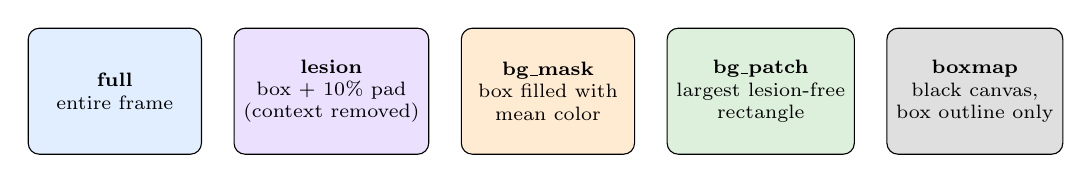
\begin{tikzpicture}[
  node distance=4mm,
  v/.style={rectangle, draw, rounded corners, minimum height=16mm, minimum width=22mm, align=center, font=\scriptsize, fill=boxwle},
  lbl/.style={font=\scriptsize\itshape}
]
  \node[v] (full) {\textbf{full}\\entire frame};
  \node[v, right=of full, fill=boxeus] (lesion) {\textbf{lesion}\\box + 10\% pad\\(context removed)};
  \node[v, right=of lesion, fill=boxhead] (bgmask) {\textbf{bg\_mask}\\box filled with\\mean color};
  \node[v, right=of bgmask, fill=boxbb] (bgpatch) {\textbf{bg\_patch}\\largest lesion-free\\rectangle};
  \node[v, right=of bgpatch, fill=gray!25] (boxmap) {\textbf{boxmap}\\black canvas,\\box outline only};
\end{tikzpicture}
\end{adjustbox}
\end{center}

\texttt{bg\_mask} is \emph{not} a clean ablation --- the filled rectangle still encodes the box's size and
position, which Experiment~1 shows is class-associated. \texttt{bg\_patch} and \texttt{boxmap} were added
to separate tissue-context leakage from pure geometry leakage; \texttt{bg\_mask} is retained only to show
the contamination it causes.

\subsection{Experiments and mechanisms tested}

\begin{center}
\begin{tabular}{L{2.6cm}L{6.3cm}L{4.6cm}}
\toprule
\textbf{Experiment} & \textbf{Question} & \textbf{Verdict} \\
\midrule
01 Dataset confounds & Is the label predictable from center, demographics, size, location, geometry? & Center: not present (Cram\'er's V 0.099) \\
02 Low-level probes & Is center or the label decodable from global color/exposure stats? & Center: present, strong (0.81 vs.\ 0.167 chance) \\
03 Lesion vs.\ background & Counterfactual ablation: remove the lesion, see what survives & Present, strong (68--95\% retained) \\
04 Cross-center & Train Center-1, test Centers 2--6 & Partial (52--100\% retained, small $n$) \\
05 Split leakage & Patient-level vs.\ image-level splitting & Present (+0.14 to +0.58 balanced acc.) \\
06 Synthesis & Collates 01--05 into one verdict table & --- \\
\bottomrule
\end{tabular}
\end{center}

\subsection{Core result (Experiment 3)}

Balanced accuracy, retention against the full-image reference in brackets:

\begin{center}
\begin{tabular}{lccccc}
\toprule
Task & chance & full & lesion & bg\_patch & boxmap \\
\midrule
WLE binary & 0.500 & 0.706 & 0.754 (123\%) & \textbf{0.695 (95\%)} & 0.598 (48\%) \\
WLE subtype & 0.200 & 0.326 & 0.448 (197\%) & \textbf{0.299 (79\%)} & 0.300 (80\%) \\
EUS binary & 0.500 & 0.679 & 0.749 (139\%) & \textbf{0.621 (68\%)} & 0.666 (93\%) \\
EUS subtype & 0.200 & 0.322 & 0.599 (326\%) & \textbf{0.292 (75\%)} & 0.431 (189\%) \\
\bottomrule
\end{tabular}
\end{center}

\subsection{Mechanism summary}

\begin{center}
\begin{tabular}{L{5.6cm}L{3.4cm}L{4.2cm}}
\toprule
\textbf{Mechanism} & \textbf{Verdict} & \textbf{Evidence} \\
\midrule
Center predicts the label & Not present & Cram\'er's V 0.099; probe lift +0.003 \\
Site encoded in pixels & Present (strong) & center decodable at 0.81 vs.\ 0.167 chance \\
Label leaks via global appearance & Not present & max probe lift +0.10 \\
Label predictable from non-lesion pixels & Present (strong) & 68--95\% retention \\
Annotation geometry alone diagnostic & Present (strong) & 48--189\% retention \\
Collapse on unseen site & Partial & 52--100\% retained, small external $n$ \\
Image-level split inflation & Present & +0.14 to +0.58 balanced accuracy \\
\bottomrule
\end{tabular}
\end{center}

\textbf{Headline:} the label is recoverable from context and box geometry, largely independent of lesion
appearance; but the site fingerprint, while real, is \emph{not} the dominant route to the label (Center-1
supplies 537/641 patients, so site and class are near-independent). \textbf{Detection is markedly less
shortcut-prone than classification}: a classifier retains 68--95\% of accuracy on lesion-free crops, while a
detector fires on the same crops only $\sim$0.3$\times$ as often as on full frames --- box regression forces
commitment to a location.

\clearpage
% =====================================================================
\section{Mitigation Study I --- Augmentation-Level (Experiment 7)}
\label{sec:mit1}
% =====================================================================

\noindent\textit{Full accuracy/balanced-accuracy for every condition/variant here: Appendix~\ref{sec:appendix-metrics}.3.}

\subsection{Methods}

\begin{center}
\begin{tabular}{lL{9.5cm}}
\toprule
\textbf{Augmentation} & \textbf{Mechanism} \\
\midrule
\texttt{scale} & Random rescale of the lesion, 0.5--1.6$\times$; targets the geometry shortcut \\
\texttt{bgswap} & Lesion pasted onto a \emph{different patient's} lesion-free background; targets the context shortcut \\
\texttt{both} & \texttt{scale} + \texttt{bgswap} composed \\
\texttt{hard negatives} & Lesion-free frames from the same patients mined into training, at a target fraction (e.g.\ 0.3) \\
\bottomrule
\end{tabular}
\end{center}

Protocol differs from Experiment 3 on purpose: \textbf{one} model is trained on ordinary frames and ablated
\emph{at inference} (``does this trained model rely on the lesion?''), rather than retraining a separate
model per input variant (``is the label learnable from this input?'').

\subsection{Classifier-level results (Experiment 7)}

Change in background reliance (\texttt{ret\_bg\_patch}) vs.\ baseline, negative = less shortcut:

\begin{center}
\begin{tabular}{lccc}
\toprule
Task & \texttt{scale} & \texttt{bgswap} & \texttt{both} \\
\midrule
WLE binary & $-0.6\%$ & \textbf{$-75.2\%$} & $-50.9\%$ \\
WLE subtype & $-46.5\%$ & $-41.2\%$ & $-42.4\%$ \\
EUS binary & $-28.7\%$ & $-30.9\%$ & $+1.0\%$ \\
EUS subtype & $+37.3\%$ & $+26.8\%$ & $+23.2\%$ \\
\bottomrule
\end{tabular}
\end{center}

\textbf{WLE responds; EUS does not.} \texttt{both} cuts WLE-binary background reliance from 69\% to 18\% for
$-0.069$ balanced accuracy; on subtype it cuts 45\% to 3\% while \emph{improving} accuracy (+0.042).
\texttt{bgswap} alone is the strongest single intervention ($-75.2\%$) but costs the most accuracy
($-0.153$). On EUS, every condition makes reliance \emph{worse} (grayscale, narrow-field ultrasound makes a
pasted lesion implausible, so the augmentation mostly injects noise).


\clearpage
% =====================================================================
\section{Mitigation Study II --- Architectural (Experiments 12--16)}
\label{sec:mit2}
% =====================================================================

\noindent\textit{Full accuracy/balanced-accuracy for every condition/seed/variant here: Appendix~\ref{sec:appendix-metrics}.3.}

Three further classifier-level mitigations, all following Experiment 7's protocol (train \emph{one} model,
ablate at inference), reusing Experiment 3's variant definitions and this project's general seed-noise-floor
discipline (see the Introduction).

\subsection{Adversarial discriminator with gradient reversal (Experiment 12)}

A shared ResNet-18 backbone feeds a main classification head (full image, ordinary cross-entropy) and a
discriminator head, behind a Gradient Reversal Layer (GRL), that tries to predict the true label from that
sample's \texttt{bg\_patch} crop alone. Reversed gradients push the backbone toward representations from
which the discriminator \emph{cannot} predict the label from shortcut-only pixels.

\begin{center}
\begin{adjustbox}{max width=\textwidth}
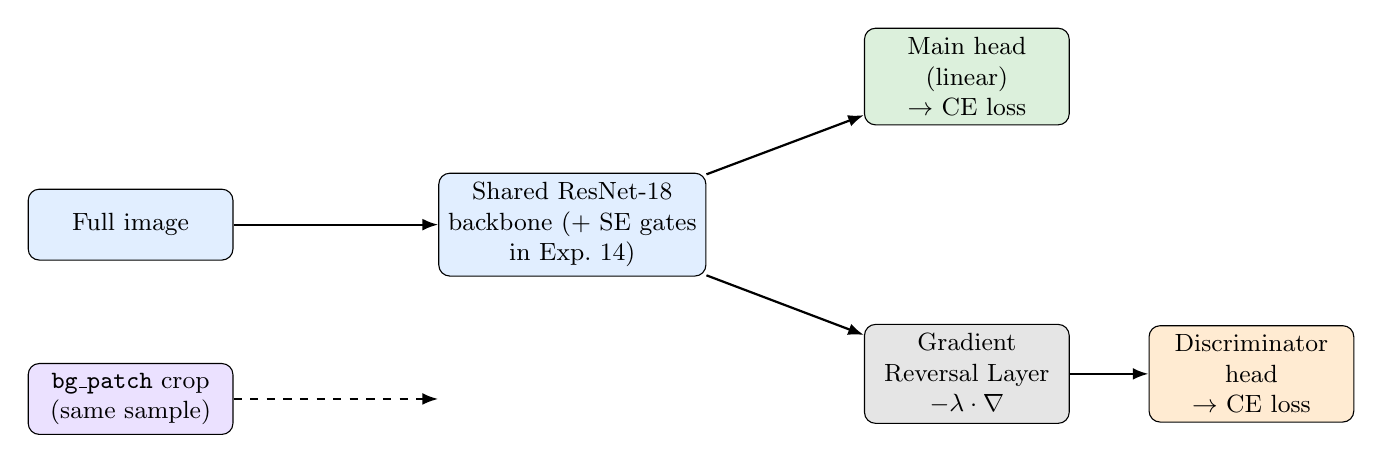
\begin{tikzpicture}[
  node distance=7mm and 9mm,
  block/.style={rectangle, draw, rounded corners, minimum height=9mm, minimum width=26mm, align=center, font=\small},
  arr/.style={-{Latex[length=2mm]}, thick}
]
  \node[block, fill=boxwle] (img) {Full image};
  \node[block, below=13mm of img, fill=boxeus] (bgp) {\texttt{bg\_patch} crop\\(same sample)};
  \node[block, right=26mm of img, fill=boxwle] (backbone) {Shared ResNet-18\\backbone (+ SE gates\\in Exp.\ 14)};
  \node[block, above right=6mm and 20mm of backbone, fill=boxbb] (main) {Main head\\(linear)\\$\to$ CE loss};
  \node[block, below right=6mm and 20mm of backbone, fill=gray!20] (grl) {Gradient\\Reversal Layer\\$-\lambda \cdot \nabla$};
  \node[block, right=10mm of grl, fill=boxhead] (disc) {Discriminator\\head\\$\to$ CE loss};

  \draw[arr] (img) -- (backbone);
  \draw[arr, dashed] (bgp) -- (backbone.west |- bgp);
  \draw[arr] (backbone) -- (main);
  \draw[arr] (backbone) -- (grl);
  \draw[arr] (grl) -- (disc);
\end{tikzpicture}
\end{adjustbox}
\end{center}

\texttt{boxmap} is a secondary, ablatable discriminator target (riskier: a synthetic near-black canvas is
out-of-distribution for a natural-image backbone). GRL $\lambda$ follows a DANN-style sigmoid ramp
($\lambda_{\max}=1.0$, 2-epoch warm-up).

\subsection{Bbox blur (Experiment 13) and channel attention (Experiment 14)}

\textbf{Bbox blur}: Gaussian-blurs everything outside a heavily feathered, generously padded ($\geq$1.15$\times$
box extent), per-sample-jittered region around the lesion box, \emph{during training only}, guarding
explicitly against the \texttt{bg\_mask} trap (a hard blur boundary would itself encode geometry).

\textbf{Channel attention}: squeeze-and-excite (SE) gates on ResNet-18's stages (simplified from
\texttt{Channel\_Att\_Bridge} in UltraLight-VM-UNet). \texttt{se\_*\_ce} (no discriminator) is an
\emph{expected-null control}; \texttt{se\_all\_adv} composes SE gates with the Experiment-12 discriminator.

\subsection{Results and verdicts}

\begin{center}
\begin{tabular}{L{2.1cm}L{7.6cm}L{4.4cm}}
\toprule
\textbf{Method} & \textbf{\texttt{ret\_bg\_patch} vs.\ baseline, 4 modality/task cells} & \textbf{Verdict} \\
\midrule
Exp.\ 12 (GRL disc.) & 7/8 conditions negative; 1/8 (EUS/subtype) cleared the noise floor & \unconf{} at 3 seeds \\
Exp.\ 13 (bbox blur) & mixed sign on WLE; \textbf{backfires on EUS binary} (+34 to +38\% retention) & \noeffect{}; no boundary-leak fired \\
Exp.\ 14 (\texttt{se\_all\_adv}) & \textbf{8/8 cells negative}, clean dose-response vs.\ \texttt{se\_layer4\_adv} & \unconf{}, most consistent direction \\
\bottomrule
\end{tabular}
\end{center}

\textbf{Exp.\ 15/16 follow-up.} \texttt{baseline} and \texttt{se\_all\_adv} extended from 3 to 7 seeds (Exp.\
15), then rerun at up to 100 epochs with early-stop patience 20 (Exp.\ 16). Models converged well before the
cap (mean 27--45 epochs). \textbf{All 4 cells still negative}, none clearing $2\times$ the pooled seed-noise
floor even after proper convergence --- noise floors actually \emph{tightened} in 3 of 4 cells. \textbf{Final
verdict: \texttt{se\_all\_adv} is a real, consistent, but small effect --- not strong enough to confirm as a
validated mitigation.} None of the three methods (12/13/14) cleared their own noise floor with the budget
tested.

\clearpage
% =====================================================================
\section{Track A --- Classification-Accuracy Campaign (\S10, \S12--\S14)}
\label{sec:tracka}
% =====================================================================

\noindent\textit{Full accuracy, balanced accuracy, precision, recall, F1, ROC-AUC, and PR-AUC for all 62 runs: Appendix~\ref{sec:appendix-metrics}.1.}

Every classification result before this section was a shortcut-learning diagnostic or a frozen-embedding
fusion component. Track~A pushes single-modality lesion classification (binary NET/non-NET, 5-way subtype)
as an end in itself, with a trainable backbone, on the same discipline as the rest of the project.

\subsection{Backbones and infrastructure}

\begin{center}
\begin{tabular}{ll}
\toprule
Backbones & \texttt{resnet50}, \texttt{convnext\_tiny}, \texttt{efficientnet\_b0}, \texttt{dinov3\_vits16} \\
Freeze modes & \texttt{none} (full fine-tune), \texttt{partial} (last blocks), \texttt{head} (frozen backbone) \\
Losses & \texttt{ce}, \texttt{weighted\_ce}, \texttt{seesaw\_ce} \\
Oversampling & \texttt{none}, \texttt{size} (size-aware RFS, threshold 0.2) \\
Image size & 224 \\
Optimizer & AdamW, lr $3\times10^{-4}$ default, batch 32 \\
Epochs & 30 default (20 for the backbone screen, early-stop patience 8) \\
Cross-validation & 5-fold, patient-grouped \\
\bottomrule
\end{tabular}
\end{center}

Every run writes per-fold loss/LR curves, a confusion matrix, and ROC/PR curves; ROC-AUC/PR-AUC are logged
alongside balanced accuracy.

\subsection{Fair-baseline gate (10.1) --- PASS}

A fine-tuned ResNet-50 must clearly beat the frozen-embedding SVM baseline used earlier in this project's
audit work (\texttt{experiments/svm\_classifier.py}, an SVM on frozen ResNet-50/DINOv3 embeddings), or the
new pipeline has a bug:

\begin{center}
\begin{tabular}{lcc}
\toprule
Task & Frozen-SVM & Fine-tuned ResNet-50 \\
\midrule
WLE binary & 0.6447 & $\mathbf{0.7616\pm0.0234}$ \\
WLE subtype & 0.2995 & $\mathbf{0.4398\pm0.0457}$ \\
\bottomrule
\end{tabular}
\end{center}

\subsection{Backbone screen (10.2)}

32 runs (4 backbones $\times$ 2 modalities $\times$ 2 tasks $\times$ \{frozen, unfrozen\}), single seed 42:

\begin{center}
\begin{tabular}{llcc}
\toprule
Modality/task & Backbone & Frozen (head) & Unfrozen (none) \\
\midrule
WLE binary & efficientnet\_b0 & 0.6724 & \textbf{0.7711} \\
WLE binary & dinov3\_vits16 & \textbf{0.7072} & 0.5711 \\
WLE subtype & efficientnet\_b0 & 0.3069 & \textbf{0.4348} \\
EUS binary & resnet50 & 0.5279 & \textbf{0.6925} \\
EUS subtype & efficientnet\_b0 & 0.2327 & \textbf{0.3602} \\
\bottomrule
\end{tabular}
\end{center}
(chance: 0.500 binary, 0.200 subtype; full 16-row table in \texttt{FINDINGS.md} \S10.2.)

\textbf{efficientnet\_b0} is the best unfrozen WLE backbone, carried into the lever screen.
\textbf{DINOv3 is the one backbone where full fine-tuning backfires} --- frozen beats unfrozen on WLE
binary (0.7072 vs.\ 0.5711) and unfrozen collapses to chance on EUS. Root cause identified in \S12.3: the
project's CNN-tuned default LR ($3\times10^{-4}$) is too high for a ViT.

\subsection{Lever screen and multi-seed confirmation (10.3--10.5)}

\texttt{weighted\_ce} on subtype: single-seed $+0.0221$, confirmed at 3 seeds
($0.4282\pm0.0127 \to 0.4609\pm0.0035$, $\Delta+0.0327$, clears floor by $\sim$2.5$\times$).
\textbf{Counterfactual gate}: \texttt{ret\_bg\_patch} 33\% (win) vs.\ 42\% (baseline) --- \textbf{lower}, so
the gain is not shortcut-driven. \confirmed{} as a validated classification-accuracy improvement.

\subsection{DINOv3 \texttt{--freeze partial} (12.2) --- new best classifier}

Unfreezing only the last 4 (of 12) transformer blocks:

\begin{center}
\begin{tabular}{lccc}
\toprule
Task & seed 42 & seed 123 & seed 7 (mean $\pm$ std) \\
\midrule
binary & 0.7963 & 0.8136 & 0.8105 $\to$ $\mathbf{0.8068\pm0.0075}$ \\
subtype & 0.4741 & 0.4899 & 0.4697 $\to$ $\mathbf{0.4779\pm0.0087}$ \\
\bottomrule
\end{tabular}
\end{center}

\confirmed{} on both tasks (binary $+0.0357$ over \texttt{efficientnet\_b0}; subtype $+0.0170$ over
\texttt{weighted\_ce}). \textbf{Counterfactual gate: PARTIAL} --- \texttt{bg\_patch} retention is technically
higher than the CNN baselines' (54\%>46\%, 40\%>33\%, a literal WARN), but retention on the
\emph{isolated-lesion} crop is dramatically higher too (87\%/83\% vs.\ 55\%/55\%) --- DINOv3's richer
representation appears to extract more signal from \emph{both} lesion and context, not to substitute
shortcut-reading for lesion-reading. Recorded as the new best result, flagged partial rather than clean.

\subsection{Compounding levers and ensembling (13.2, 13.4)}

DINOv3-partial + \texttt{weighted\_ce} on subtype \confirmed{} at 3 seeds ($0.4957\pm0.0033$, gate clean:
\texttt{bg\_patch} retention \emph{dropped} 40\%$\to$27\%). Multi-seed probability ensembling (3 already-trained
seeds, zero extra GPU time) reaches new campaign bests:

\begin{center}
\begin{tabular}{lccc}
\toprule
Config & seed mean $\pm$ std & Ensemble & $\Delta$ \\
\midrule
DINOv3-partial, binary & $0.8063\pm0.0078$ & \textbf{0.8209} & +0.0146 \\
DINOv3-partial + weighted\_ce, subtype & $0.4988\pm0.0049$ & \textbf{0.5230} & +0.0242 \\
\bottomrule
\end{tabular}
\end{center}

\subsection{EUS: treat as shortcut-suspect by default}

Extending the counterfactual gate to the remaining 17 EUS backbone-screen checkpoints found retentions from
$-43\%$ to \textbf{89\%} (\texttt{efficientnet\_b0}/subtype/frozen) --- close to the $\sim$100\% ``pure
shortcut'' DINOv3-EUS precedent from the audit. \textbf{No EUS classification result in this campaign is
both strong and counterfactually clean}; the single new-best EUS classifier that does clear the gate
cleanly is DINOv3 \texttt{--freeze partial} (\S14.3): binary $0.7386\pm0.0313$ (35\% \texttt{bg\_patch}
retention), subtype $0.3764\pm0.0507$ (15\% retention).

\subsection{Closed threads: TTA and DINOv3 fine-tuning LR}

Flip-TTA (12.4) and 5-crop TTA (14.6) are both null on every checkpoint tried: training already includes
\texttt{RandomHorizontalFlip}/\texttt{RandomResizedCrop}, leaving TTA nothing new to add.
\texttt{unfreeze\_last\_n} sweep (14.5): $n=6$--8 modestly beats the default $n=4$ (single-seed, not
confirmed); even $n=12$ avoids catastrophic collapse because the patch/position embeddings stay frozen under
\texttt{--freeze partial} regardless of $n$ --- the actual reason \texttt{--freeze none} was catastrophic
(\S10.2) while a much lower LR (\S12.3, $10^{-5}$) recovers most of the gap.

\clearpage
% =====================================================================
\section{Joint End-to-End Two-Tower WLE+EUS Fusion (\S15)}
\label{sec:fusion2}
% =====================================================================

\noindent\textit{Accuracy, balanced accuracy, and macro-F1 for all 69 run/ablation combinations: Appendix~\ref{sec:appendix-metrics}.2.}

Every prior fusion result trained \texttt{FusionHead} on \textbf{frozen, pre-extracted, single-pass}
features --- the per-modality backbones never see a fusion-loss gradient, and no image augmentation happens
in the fusion stage. This architecture is structurally different: two independently trainable backbones,
jointly fine-tuned end-to-end, with independent per-modality augmentation every training step.

\subsection{Architecture}

\begin{center}
\begin{adjustbox}{max width=\textwidth}
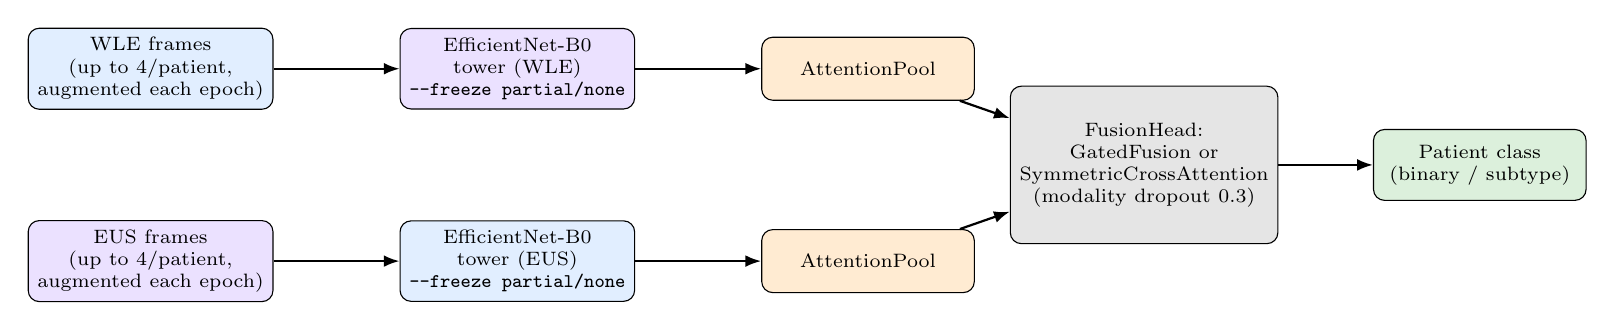
\begin{tikzpicture}[
  node distance=7mm and 9mm,
  block/.style={rectangle, draw, rounded corners, minimum height=9mm, minimum width=27mm, align=center, font=\scriptsize},
  arr/.style={-{Latex[length=2mm]}, thick}
]
  \node[block, fill=boxwle] (wle) {WLE frames\\(up to 4/patient,\\augmented each epoch)};
  \node[block, below=14mm of wle, fill=boxeus] (eus) {EUS frames\\(up to 4/patient,\\augmented each epoch)};
  \node[block, right=16mm of wle, fill=boxeus] (twle) {EfficientNet-B0\\tower (WLE)\\\texttt{--freeze partial/none}};
  \node[block, right=16mm of eus, fill=boxwle] (teus) {EfficientNet-B0\\tower (EUS)\\\texttt{--freeze partial/none}};
  \node[block, right=16mm of twle, minimum height=8mm, fill=boxhead] (poolw) {AttentionPool};
  \node[block, right=16mm of teus, minimum height=8mm, fill=boxhead] (poole) {AttentionPool};
  \node[block, right=18mm of $(poolw)!0.5!(poole)$, minimum height=20mm, fill=gray!20] (fuse) {FusionHead:\\GatedFusion or\\SymmetricCrossAttention\\(modality dropout 0.3)};
  \node[block, right=12mm of fuse, fill=boxbb] (out) {Patient class\\(binary / subtype)};

  \draw[arr] (wle) -- (twle);
  \draw[arr] (eus) -- (teus);
  \draw[arr] (twle) -- (poolw);
  \draw[arr] (teus) -- (poole);
  \draw[arr] (poolw) -- (fuse);
  \draw[arr] (poole) -- (fuse);
  \draw[arr] (fuse) -- (out);
\end{tikzpicture}
\end{adjustbox}
\end{center}

\begin{sloppypar}
Two independent \texttt{efficientnet\_b0} towers (ImageNet-pretrained; \texttt{--freeze partial} unfreezes
the last two \texttt{features} stages) feed the \textbf{unmodified} \texttt{cadsel.fusion.FusionHead}
module: an attention-weighted pool over each modality's frames, then a \texttt{GatedFusion} or
\texttt{SymmetricCrossAttentionFusion} combination layer, with modality dropout and missing-modality
masking. One joint model per fold is
trained with \texttt{modality\_dropout=0.3} throughout, and \texttt{wle\_only} / \texttt{eus\_only} /
\texttt{fused} are reported as three masked-inference views of that single model.
\end{sloppypar}

\subsection{Hyperparameters}

\begin{center}
\begin{tabular}{lL{10cm}}
\toprule
Towers & \texttt{efficientnet\_b0} $\times$ 2 (independent weights) \\
Frame budget & up to 4 frames/patient/modality, sampled with replacement \\
Loss & \texttt{weighted\_ce} \\
Fusion & \texttt{gated} (default) or \texttt{symmetric} \\
Learning rate & flat $10^{-4}$, or discriminative (backbone $10^{-5}$ / head $10^{-4}$) \\
Epochs & 30 (initial screen) or 100 / patience 20 (confirmed configs) \\
Cross-validation & 5-fold, patient-grouped \\
Optional levers & \texttt{--lesion-crop} (crop to box + 10\% pad, pre-augmentation), \texttt{--bg-remove-prob} (stochastic mean-fill outside the box) \\
\bottomrule
\end{tabular}
\end{center}

\subsection{Binary task: confirmed fusion win}

\begin{center}
\begin{tabular}{llccc}
\toprule
Config & Ablation (denom.) & seed 42/123/7 & \textbf{3-seed mean $\pm$ std} \\
\midrule
\texttt{--freeze partial}, flat LR & wle\_only (unpaired) & 0.687/0.722/0.737 & $0.7153\pm0.0208$ \\
& \textbf{fused} (unpaired) & 0.749/0.761/0.769 & $\mathbf{0.7596\pm0.0082}$ \\
\texttt{--freeze none} & wle\_only (unpaired) & 0.766/0.773/0.754 & $0.7644\pm0.0093$ \\
& \textbf{fused} (unpaired) & 0.803/0.808/0.792 & $\mathbf{0.8007\pm0.0067}$ \\
\texttt{--freeze none} + \texttt{--lesion-crop} & wle\_only (unpaired) & 0.769/0.768/0.783 & $0.7733\pm0.0071$ \\
& eus\_only (paired) & 0.682/0.725/0.710 & $0.7057\pm0.0178$ \\
& \textbf{fused} (unpaired) & 0.817/0.794/0.822 & $\mathbf{0.8110\pm0.0123}$ \\
\bottomrule
\end{tabular}
\end{center}

\textbf{\texttt{fused} vs.\ \texttt{wle\_only}} (within \texttt{--freeze none}): $\Delta+0.0363$, noise floor
$\approx0.0115$ --- \confirmed{}, $\sim$3.2$\times$ the floor, the cleanest margin in this section.
\textbf{\texttt{--freeze none} vs.\ \texttt{--freeze partial}}, both fused: $\Delta+0.0411$, floor
$\approx0.0106$ --- \confirmed{}. \texttt{--lesion-crop} confirms a real EUS-only gain
($0.6197\pm0.0216 \to 0.7057\pm0.0178$, $\Delta+0.0860$, $\sim$3.1$\times$ floor) but its \texttt{fused}
delta over plain \texttt{--freeze none} ($+0.0103$) does \emph{not} clear its own floor ($\approx0.0140$) ---
a real single-modality win that does not (yet) propagate to the headline fused metric, plausibly because
\texttt{GatedFusion}'s gate structurally favors WLE.

\textbf{Multi-seed ensembling} (zero extra training) reaches campaign-best fused/unpaired balanced accuracy
of \textbf{0.8219} (\texttt{--lesion-crop} ensemble) / 0.8160 (\texttt{--freeze none} ensemble alone).

\subsection{Counterfactual gate --- PASSED}

Built \texttt{36\_joint\_fusion\_counterfactual.py}, the patient-level, multi-frame, two-modality adaptation
of the classifier gate; swaps both towers to the same variant simultaneously per patient. Run against the
confirmed \texttt{--freeze none} seed-42 checkpoint:

\begin{center}
\begin{tabular}{lcc}
\toprule
Variant & balanced accuracy & retention vs.\ full \\
\midrule
full (real images, both towers) & 0.803 & --- \\
lesion (crop to box + padding) & 0.632 & 44\% \\
bg\_mask (lesion erased, background kept) & 0.644 & 48\% \\
bg\_patch (pure background, no lesion) & 0.627 & 42\% \\
\textbf{boxmap} (black canvas, box outline only) & \textbf{0.494} & \textbf{$-2\%$} \\
\bottomrule
\end{tabular}
\end{center}

With every trace of real tissue removed, balanced accuracy falls to essentially exact chance (0.494 vs.\
0.500). \textbf{Gate PASSED}: the confirmed win is genuine lesion-dependent signal, not shortcut-reading.

\subsection{Subtype task: confirmed on the unpaired denominator}

\begin{center}
\begin{tabular}{llccc}
\toprule
Config & Ablation & seed 42/123/7 & \textbf{3-seed mean $\pm$ std} \\
\midrule
discriminative LR, \texttt{--freeze partial} & wle\_only (unpaired) & 0.464/0.445/0.502 & $0.4704\pm0.0234$ \\
& \textbf{fused} (unpaired) & 0.510/0.481/0.528 & $\mathbf{0.5063\pm0.0193}$ \\
\texttt{--freeze none} + \texttt{--lesion-crop} & wle\_only (unpaired) & 0.527/0.469/0.518 & $0.5049\pm0.0254$ \\
& \textbf{fused} (unpaired) & 0.555/0.514/0.557 & $\mathbf{0.5419\pm0.0201}$ \\
\bottomrule
\end{tabular}
\end{center}

Unpaired balanced accuracy delta $+0.0359$ vs.\ floor $\approx0.0304$ (1.18$\times$, tight but real; macro-F1
cross-check confirms more cleanly at 2.9$\times$). \texttt{--lesion-crop} on \texttt{--freeze none} then
confirms a \textbf{new subtype best} ($0.5419\pm0.0201$, $\Delta+0.0356$ over the prior best, $\sim$1.28$\times$
floor). Counterfactual gate on the discriminative-LR checkpoint \textbf{PASSED} (boxmap retention 2\%,
essentially chance). \textbf{Caveat}: the paired-only denominator's confirmation is razor-thin (clears its
floor by 0.0002) and should not be leaned on.

\subsection{Negative and null screens}

Discriminative backbone LR (\S15.3) helped \texttt{wle\_only} more than \texttt{fused}, narrowing rather than
widening the fusion gap --- a useful negative, not carried forward. \texttt{--fusion symmetric} (\S15.7) is
within noise of gated and does not let lesion-crop's EUS gain reach the fused output either, refuting the
specific ``WLE-bias'' hypothesis. \texttt{--bg-remove-prob 0.5} (\S15.9) is clearly negative (fused
$-0.0397$), single-seed, not escalated: stochastic mean-filling followed by \texttt{RandomResizedCrop} can
land entirely inside the filled region, producing noisy supervision rather than useful regularization.

\clearpage
% =====================================================================
\section{Cross-Cutting Summary}
\label{sec:summary}
% =====================================================================

\subsection{Campaign-best numbers}

\begin{center}
\begin{tabular}{L{4.3cm}L{7.4cm}C{2.6cm}}
\toprule
\textbf{Line of work} & \textbf{Best confirmed configuration} & \textbf{Score} \\
\midrule
Track A, WLE binary & DINOv3-partial, 3-seed ensemble & 0.8209 bal.\ acc. \\
Track A, WLE subtype & DINOv3-partial + weighted\_ce, 3-seed ensemble & 0.5230 bal.\ acc. \\
Track A, EUS binary (gate-clean) & DINOv3-partial & 0.7386 $\pm$ 0.0313 bal.\ acc. \\
Joint fusion, binary & \texttt{--freeze none} + \texttt{--lesion-crop}, ensemble & 0.8219 bal.\ acc. \\
Joint fusion, subtype & \texttt{--freeze none} + \texttt{--lesion-crop} & 0.5419 $\pm$ 0.0201 bal.\ acc. \\
\bottomrule
\end{tabular}
\end{center}

\subsection{Confirmed levers across the whole project}

\begin{center}
\begin{tabular}{L{6.8cm}L{6.2cm}}
\toprule
\textbf{Confirmed positive} & \textbf{Confirmed negative} \\
\midrule
\texttt{weighted\_ce} loss, WLE subtype (Track A) & DINOv3 \texttt{--freeze none} at the project's default LR (Track A) \\
DINOv3 \texttt{--freeze partial} (Track A, both WLE tasks) & Flip-TTA / 5-crop TTA (Track A) \\
Multi-seed probability ensembling (Track A \& joint fusion) & \texttt{--bg-remove-prob} (joint fusion) \\
Joint two-tower fusion, binary (\texttt{--freeze none}) & \\
Joint two-tower fusion, subtype (unpaired denominator) & \\
\texttt{--lesion-crop}, EUS single-modality signal & \\
\bottomrule
\end{tabular}
\end{center}

\subsection{Standing cautions}

\begin{itemize}[nosep]
  \item \textbf{EUS classification results are shortcut-suspect by default} unless individually gated ---
    only DINOv3-partial (\S14.3) is both strong and clean.
  \item \textbf{A clean confirmation and a clean counterfactual pass are two different bars.} DINOv3-partial
    is a confirmed win on both WLE tasks (Section~\ref{sec:tracka}) yet only flags PARTIAL on its own
    counterfactual gate --- a result can clear the noise floor without being unambiguously shortcut-free.
  \item \textbf{A confirmation can be real and still be razor-thin.} The joint-fusion subtype win on the
    paired-only denominator (Section~\ref{sec:fusion2}) clears its own noise floor by only 0.0002 --- treat
    it as directionally right, not as statistically solid as the unpaired-denominator result next to it.
\end{itemize}

\clearpage
% =====================================================================
\section{Implementation Lessons}
\label{sec:lessons}
% =====================================================================

\begin{itemize}[nosep]
  \item \textbf{Run-name collisions silently overwrite results.} Any CLI flag that can distinguish two
    otherwise-identical configs must be part of the output filename, or a later run can destroy an earlier
    one's checkpoints/JSON with no error --- seen twice in this project's classification work: a learning-rate
    sweep silently overwrote Track~A's original DINOv3 \texttt{--freeze none} failure JSON (\S12.3) until
    \texttt{--lr} was added to the run-name template, and the joint-fusion multi-seed ensemble script
    initially keyed its output only on task, so a second ensemble run overwrote the first's result file
    (\S15.5) until the script was fixed to key on the full ensembled config.
\end{itemize}

\clearpage
% =====================================================================
\section{Open Items}
\label{sec:open}
% =====================================================================

\begin{itemize}[nosep]
  \item A repeated-CV or bootstrapped-confidence-interval protocol for the DINOv3-classifier-backbone
    fusion rebuild (a frozen-feature variant distinct from the trainable two-tower architecture in
    Section~\ref{sec:fusion2}), whose paired-patient pool is too small for a single 5-fold split to give a
    stable read.
  \item A counterfactual-gate adaptation for \texttt{--lesion-crop}-trained joint-fusion checkpoints (the
    model never sees uncropped content, so the existing raw-frame gate would confound distribution shift
    with genuine lesion-dependence).
  \item Domain-specific backbone pretraining (GastroNet-5M is in-domain for WLE but gated behind a
    commercial platform; no publicly downloadable SEL dataset currently exists per the paper's own Table~1
    comparison).
\end{itemize}

\clearpage
% =====================================================================
\section*{References}
\addcontentsline{toc}{section}{References}
% =====================================================================

\begin{itemize}[nosep]
\item Xu, L., Chen, S., Li, C. et al. \textit{CAD-SEL: A dual-modal colonoscopy dataset of subepithelial
  lesion.} Scientific Data (2026). doi:10.1038/s41597-026-07331-y
\item Geirhos, R. et al. \textit{Shortcut learning in deep neural networks.} Nature Machine Intelligence
  (2020).
\item Ganin, Y. \& Lempitsky, V. \textit{Unsupervised domain adaptation by backpropagation (gradient
  reversal / DANN).} ICML (2015).
\item Wang, J. et al. \textit{Seesaw Loss for Long-Tailed Instance Segmentation.} CVPR (2021).
\end{itemize}

\clearpage
\appendix
% =====================================================================
\section{Full Metrics by Run}
\label{sec:appendix-metrics}
% =====================================================================

Every table in the main text reports the headline metric(s) actually used to reach each verdict (balanced
accuracy), matching how the underlying experiments were designed and gated. This appendix reports
\textbf{accuracy, balanced accuracy, precision, recall, F1, ROC-AUC, and PR-AUC for every individual
classification run} referenced anywhere in this report, extracted programmatically from the project's own
saved result files (never re-derived by hand, to avoid transcription error at this scale). Two honesty
rules govern every cell below:

\begin{itemize}[nosep]
  \item A metric is populated only if the underlying JSON actually contains it, or is exactly derivable
    from something it contains (precision/recall/F1 from a saved confusion matrix). A cell reading
    \nl{} means \textbf{not logged} by the original experiment --- the script that produced that run
    never computed or saved that statistic, and no attempt is made to estimate it.
\end{itemize}

\subsection{Track A classifiers (Section~\ref{sec:tracka}) --- 62 runs}

The only line of work in this project with all 7 metrics natively logged per run: accuracy, balanced
accuracy, ROC-AUC, and PR-AUC come directly from \texttt{experiments/finetune\_classifier.py}'s own
evaluation code; precision and recall are macro-averaged from each run's saved 5-fold-pooled confusion
matrix.

\begingroup\footnotesize
\setlength{\tabcolsep}{3pt}
\begin{longtable}{L{4.3cm}ccccccc}
\caption{Track~A classifier runs: full 7-metric breakdown, extracted directly from each run's saved result JSON (\texttt{experiments/results/classifier\_runs/*.json}). Precision/recall/F1 are macro-averaged over classes, derived from each run's own saved confusion matrix (5-fold pooled). Accuracy and balanced accuracy are the 5-fold mean $\pm$ std; ROC-AUC and PR-AUC are the 5-fold mean (per-fold std not separately saved).}\label{tab:app-tracka}\\
\toprule
\textbf{Run} & \textbf{Acc.} & \textbf{Bal.\ Acc.} & \textbf{Prec.} & \textbf{Rec.} & \textbf{F1} & \textbf{ROC-AUC} & \textbf{PR-AUC} \\
\midrule
\endfirsthead
\toprule
\textbf{Run} & \textbf{Acc.} & \textbf{Bal.\ Acc.} & \textbf{Prec.} & \textbf{Rec.} & \textbf{F1} & \textbf{ROC-AUC} & \textbf{PR-AUC} \\
\midrule
\endhead
\texttt{\scriptsize \seqsplit{convnext\_tiny/EUS/binary/freeze-head/os-none/loss-ce/s42}} & 0.792$\pm$0.046 & 0.583$\pm$0.057 & 0.770 & 0.577 & 0.579 & 0.623 & 0.410 \\
\texttt{\scriptsize \seqsplit{convnext\_tiny/EUS/binary/freeze-none/os-none/loss-ce/s42}} & 0.771$\pm$0.020 & 0.692$\pm$0.036 & 0.686 & 0.700 & 0.692 & 0.753 & 0.508 \\
\texttt{\scriptsize \seqsplit{dinov3\_vits16/EUS/binary/freeze-head/os-none/loss-ce/s42}} & 0.778$\pm$0.044 & 0.531$\pm$0.039 & 0.871 & 0.529 & 0.492 & 0.600 & 0.389 \\
\texttt{\scriptsize \seqsplit{dinov3\_vits16/EUS/binary/freeze-none/os-none/loss-ce/s42}} & 0.765$\pm$0.038 & 0.500$\pm$0.000 & 0.382 & 0.500 & 0.433 & 0.538 & 0.263 \\
\texttt{\scriptsize \seqsplit{dinov3\_vits16/EUS/binary/freeze-partial/os-none/loss-ce/s42}} & 0.786$\pm$0.024 & 0.739$\pm$0.031 & 0.711 & 0.735 & 0.720 & 0.782 & 0.589 \\
\texttt{\scriptsize \seqsplit{efficientnet\_b0/EUS/binary/freeze-head/os-none/loss-ce/s42}} & 0.767$\pm$0.037 & 0.576$\pm$0.028 & 0.654 & 0.580 & 0.587 & 0.672 & 0.397 \\
\texttt{\scriptsize \seqsplit{efficientnet\_b0/EUS/binary/freeze-none/os-none/loss-ce/bgswap/s42}} & 0.770$\pm$0.027 & 0.682$\pm$0.044 & 0.680 & 0.675 & 0.678 & 0.753 & 0.526 \\
\texttt{\scriptsize \seqsplit{efficientnet\_b0/EUS/binary/freeze-none/os-none/loss-ce/s42}} & 0.791$\pm$0.029 & 0.684$\pm$0.033 & 0.705 & 0.681 & 0.691 & 0.731 & 0.543 \\
\texttt{\scriptsize \seqsplit{resnet50/EUS/binary/freeze-head/os-none/loss-ce/s42}} & 0.771$\pm$0.031 & 0.528$\pm$0.019 & 0.698 & 0.530 & 0.500 & 0.601 & 0.361 \\
\texttt{\scriptsize \seqsplit{resnet50/EUS/binary/freeze-none/os-none/loss-ce/s42}} & 0.782$\pm$0.050 & 0.693$\pm$0.021 & 0.700 & 0.695 & 0.697 & 0.768 & 0.563 \\
\texttt{\scriptsize \seqsplit{convnext\_tiny/EUS/subtype/freeze-head/os-none/loss-ce/s42}} & 0.691$\pm$0.061 & 0.241$\pm$0.029 & 0.262 & 0.238 & 0.229 & 0.616 & 0.303 \\
\texttt{\scriptsize \seqsplit{convnext\_tiny/EUS/subtype/freeze-none/os-none/loss-ce/s42}} & 0.684$\pm$0.058 & 0.330$\pm$0.020 & 0.359 & 0.322 & 0.327 & 0.677 & 0.363 \\
\texttt{\scriptsize \seqsplit{dinov3\_vits16/EUS/subtype/freeze-head/os-none/loss-ce/s42}} & 0.693$\pm$0.044 & 0.205$\pm$0.011 & 0.338 & 0.205 & 0.173 & 0.497 & 0.238 \\
\texttt{\scriptsize \seqsplit{dinov3\_vits16/EUS/subtype/freeze-none/os-none/loss-ce/s42}} & 0.674$\pm$0.038 & 0.233$\pm$0.045 & 0.252 & 0.227 & 0.214 & 0.524 & 0.247 \\
\texttt{\scriptsize \seqsplit{dinov3\_vits16/EUS/subtype/freeze-partial/os-none/loss-ce/s42}} & 0.672$\pm$0.034 & 0.376$\pm$0.051 & 0.405 & 0.380 & 0.387 & 0.719 & 0.395 \\
\texttt{\scriptsize \seqsplit{efficientnet\_b0/EUS/subtype/freeze-head/os-none/loss-ce/s42}} & 0.675$\pm$0.041 & 0.233$\pm$0.008 & 0.288 & 0.232 & 0.224 & 0.609 & 0.284 \\
\texttt{\scriptsize \seqsplit{efficientnet\_b0/EUS/subtype/freeze-none/os-none/loss-ce/bgswap/s42}} & 0.669$\pm$0.038 & 0.371$\pm$0.028 & 0.384 & 0.372 & 0.372 & 0.669 & 0.375 \\
\texttt{\scriptsize \seqsplit{efficientnet\_b0/EUS/subtype/freeze-none/os-none/loss-ce/s42}} & 0.662$\pm$0.043 & 0.360$\pm$0.029 & 0.410 & 0.366 & 0.383 & 0.679 & 0.392 \\
\texttt{\scriptsize \seqsplit{resnet50/EUS/subtype/freeze-head/os-none/loss-ce/s42}} & 0.690$\pm$0.042 & 0.200$\pm$0.000 & 0.138 & 0.200 & 0.163 & 0.481 & 0.205 \\
\texttt{\scriptsize \seqsplit{resnet50/EUS/subtype/freeze-none/os-none/loss-ce/s42}} & 0.665$\pm$0.049 & 0.359$\pm$0.025 & 0.417 & 0.359 & 0.368 & 0.652 & 0.364 \\
\texttt{\scriptsize \seqsplit{convnext\_tiny/WLE/binary/freeze-head/os-none/loss-ce/s42}} & 0.773$\pm$0.015 & 0.692$\pm$0.029 & 0.745 & 0.692 & 0.707 & 0.777 & 0.682 \\
\texttt{\scriptsize \seqsplit{convnext\_tiny/WLE/binary/freeze-none/os-none/loss-ce/s42}} & 0.791$\pm$0.022 & 0.761$\pm$0.030 & 0.755 & 0.760 & 0.758 & 0.842 & 0.735 \\
\texttt{\scriptsize \seqsplit{dinov3\_vits16/WLE/binary/freeze-head/os-none/loss-ce/s42}} & 0.795$\pm$0.026 & 0.707$\pm$0.044 & 0.787 & 0.708 & 0.727 & 0.800 & 0.712 \\
\texttt{\scriptsize \seqsplit{dinov3\_vits16/WLE/binary/freeze-none/os-none/loss-ce/lr1e-05/s42}} & 0.814$\pm$0.024 & 0.776$\pm$0.027 & 0.782 & 0.776 & 0.779 & 0.857 & 0.778 \\
\texttt{\scriptsize \seqsplit{dinov3\_vits16/WLE/binary/freeze-partial/os-none/loss-ce/s7}} & 0.834$\pm$0.013 & 0.810$\pm$0.015 & 0.805 & 0.810 & 0.807 & 0.883 & 0.822 \\
\texttt{\scriptsize \seqsplit{dinov3\_vits16/WLE/binary/freeze-partial/os-none/loss-ce/s42}} & 0.822$\pm$0.022 & 0.796$\pm$0.019 & 0.790 & 0.795 & 0.793 & 0.883 & 0.814 \\
\texttt{\scriptsize \seqsplit{dinov3\_vits16/WLE/binary/freeze-partial/os-none/loss-ce/unfreeze12/s42}} & 0.805$\pm$0.015 & 0.767$\pm$0.018 & 0.772 & 0.767 & 0.769 & 0.851 & 0.769 \\
\texttt{\scriptsize \seqsplit{dinov3\_vits16/WLE/binary/freeze-partial/os-none/loss-ce/unfreeze2/s42}} & 0.821$\pm$0.019 & 0.797$\pm$0.012 & 0.789 & 0.796 & 0.792 & 0.878 & 0.805 \\
\texttt{\scriptsize \seqsplit{dinov3\_vits16/WLE/binary/freeze-partial/os-none/loss-ce/unfreeze6/s42}} & 0.826$\pm$0.022 & 0.807$\pm$0.013 & 0.795 & 0.806 & 0.800 & 0.891 & 0.822 \\
\texttt{\scriptsize \seqsplit{dinov3\_vits16/WLE/binary/freeze-partial/os-none/loss-ce/unfreeze8/s42}} & 0.835$\pm$0.007 & 0.808$\pm$0.014 & 0.807 & 0.808 & 0.807 & 0.888 & 0.825 \\
\texttt{\scriptsize \seqsplit{dinov3\_vits16/WLE/binary/freeze-partial/os-none/loss-ce/s123}} & 0.843$\pm$0.028 & 0.814$\pm$0.045 & 0.816 & 0.813 & 0.815 & 0.893 & 0.828 \\
\texttt{\scriptsize \seqsplit{dinov3\_vits16/WLE/binary/freeze-partial/os-none/loss-weighted\_ce/s42}} & 0.809$\pm$0.030 & 0.801$\pm$0.011 & 0.777 & 0.801 & 0.786 & 0.880 & 0.810 \\
\texttt{\scriptsize \seqsplit{efficientnet\_b0/WLE/binary/freeze-head/os-none/loss-ce/s42}} & 0.760$\pm$0.029 & 0.672$\pm$0.046 & 0.725 & 0.672 & 0.685 & 0.753 & 0.641 \\
\texttt{\scriptsize \seqsplit{efficientnet\_b0/WLE/binary/freeze-none/os-none/loss-ce/bgswap/s42}} & 0.775$\pm$0.017 & 0.740$\pm$0.021 & 0.737 & 0.740 & 0.739 & 0.814 & 0.710 \\
\texttt{\scriptsize \seqsplit{efficientnet\_b0/WLE/binary/freeze-none/os-none/loss-ce/s42}} & 0.800$\pm$0.028 & 0.771$\pm$0.042 & 0.766 & 0.771 & 0.768 & 0.837 & 0.750 \\
\texttt{\scriptsize \seqsplit{efficientnet\_b0/WLE/binary/freeze-none/os-size/loss-ce/s42}} & 0.809$\pm$0.013 & 0.764$\pm$0.027 & 0.779 & 0.764 & 0.771 & 0.841 & 0.762 \\
\texttt{\scriptsize \seqsplit{efficientnet\_b0/WLE/binary/freeze-none/os-none/loss-seesaw\_ce/s42}} & 0.808$\pm$0.028 & 0.760$\pm$0.038 & 0.778 & 0.761 & 0.768 & 0.836 & 0.762 \\
\texttt{\scriptsize \seqsplit{efficientnet\_b0/WLE/binary/freeze-none/os-none/loss-weighted\_ce/s42}} & 0.787$\pm$0.016 & 0.764$\pm$0.021 & 0.752 & 0.764 & 0.757 & 0.841 & 0.757 \\
\texttt{\scriptsize \seqsplit{resnet50/WLE/binary/freeze-head/os-none/loss-ce/s42}} & 0.773$\pm$0.015 & 0.667$\pm$0.042 & 0.768 & 0.667 & 0.684 & 0.739 & 0.648 \\
\texttt{\scriptsize \seqsplit{resnet50/WLE/binary/freeze-none/os-none/loss-ce/s42}} & 0.795$\pm$0.031 & 0.767$\pm$0.028 & 0.760 & 0.766 & 0.763 & 0.836 & 0.732 \\
\texttt{\scriptsize \seqsplit{convnext\_tiny/WLE/subtype/freeze-head/os-none/loss-ce/s42}} & 0.693$\pm$0.016 & 0.322$\pm$0.025 & 0.451 & 0.322 & 0.318 & 0.700 & 0.384 \\
\texttt{\scriptsize \seqsplit{convnext\_tiny/WLE/subtype/freeze-none/os-none/loss-ce/s42}} & 0.637$\pm$0.038 & 0.433$\pm$0.026 & 0.422 & 0.430 & 0.422 & 0.763 & 0.446 \\
\texttt{\scriptsize \seqsplit{dinov3\_vits16/WLE/subtype/freeze-head/os-none/loss-ce/s42}} & 0.700$\pm$0.021 & 0.311$\pm$0.026 & 0.502 & 0.311 & 0.298 & 0.718 & 0.406 \\
\texttt{\scriptsize \seqsplit{dinov3\_vits16/WLE/subtype/freeze-none/os-none/loss-ce/lr1e-05/s42}} & 0.703$\pm$0.009 & 0.439$\pm$0.011 & 0.464 & 0.436 & 0.440 & 0.763 & 0.474 \\
\texttt{\scriptsize \seqsplit{dinov3\_vits16/WLE/subtype/freeze-partial/os-none/loss-ce/s7}} & 0.707$\pm$0.042 & 0.470$\pm$0.031 & 0.472 & 0.474 & 0.469 & 0.785 & 0.500 \\
\texttt{\scriptsize \seqsplit{dinov3\_vits16/WLE/subtype/freeze-partial/os-none/loss-ce/s42}} & 0.689$\pm$0.034 & 0.474$\pm$0.033 & 0.487 & 0.474 & 0.479 & 0.788 & 0.504 \\
\texttt{\scriptsize \seqsplit{dinov3\_vits16/WLE/subtype/freeze-partial/os-none/loss-ce/s123}} & 0.699$\pm$0.031 & 0.490$\pm$0.054 & 0.498 & 0.491 & 0.491 & 0.782 & 0.491 \\
\texttt{\scriptsize \seqsplit{dinov3\_vits16/WLE/subtype/freeze-partial/os-none/loss-weighted\_ce/s7}} & 0.528$\pm$0.045 & 0.494$\pm$0.030 & 0.402 & 0.492 & 0.418 & 0.770 & 0.471 \\
\texttt{\scriptsize \seqsplit{dinov3\_vits16/WLE/subtype/freeze-partial/os-none/loss-weighted\_ce/s42}} & 0.574$\pm$0.089 & 0.500$\pm$0.025 & 0.445 & 0.503 & 0.460 & 0.779 & 0.485 \\
\texttt{\scriptsize \seqsplit{dinov3\_vits16/WLE/subtype/freeze-partial/os-none/loss-weighted\_ce/s123}} & 0.585$\pm$0.095 & 0.493$\pm$0.036 & 0.428 & 0.502 & 0.449 & 0.782 & 0.470 \\
\texttt{\scriptsize \seqsplit{efficientnet\_b0/WLE/subtype/freeze-head/os-none/loss-ce/s42}} & 0.678$\pm$0.013 & 0.307$\pm$0.026 & 0.398 & 0.306 & 0.299 & 0.683 & 0.364 \\
\texttt{\scriptsize \seqsplit{efficientnet\_b0/WLE/subtype/freeze-none/os-none/loss-ce/s7}} & 0.675$\pm$0.025 & 0.410$\pm$0.022 & 0.448 & 0.406 & 0.418 & 0.728 & 0.434 \\
\texttt{\scriptsize \seqsplit{efficientnet\_b0/WLE/subtype/freeze-none/os-none/loss-ce/bgswap/s42}} & 0.641$\pm$0.038 & 0.432$\pm$0.030 & 0.437 & 0.430 & 0.431 & 0.746 & 0.449 \\
\texttt{\scriptsize \seqsplit{efficientnet\_b0/WLE/subtype/freeze-none/os-none/loss-ce/s42}} & 0.677$\pm$0.016 & 0.435$\pm$0.050 & 0.447 & 0.433 & 0.431 & 0.743 & 0.466 \\
\texttt{\scriptsize \seqsplit{efficientnet\_b0/WLE/subtype/freeze-none/os-none/loss-ce/s123}} & 0.673$\pm$0.030 & 0.439$\pm$0.030 & 0.469 & 0.440 & 0.448 & 0.747 & 0.454 \\
\texttt{\scriptsize \seqsplit{efficientnet\_b0/WLE/subtype/freeze-none/os-size/loss-ce/s42}} & 0.668$\pm$0.013 & 0.416$\pm$0.037 & 0.438 & 0.413 & 0.417 & 0.748 & 0.437 \\
\texttt{\scriptsize \seqsplit{efficientnet\_b0/WLE/subtype/freeze-none/os-none/loss-seesaw\_ce/s42}} & 0.691$\pm$0.016 & 0.413$\pm$0.041 & 0.452 & 0.415 & 0.419 & 0.750 & 0.454 \\
\texttt{\scriptsize \seqsplit{efficientnet\_b0/WLE/subtype/freeze-none/os-none/loss-weighted\_ce/s7}} & 0.581$\pm$0.067 & 0.466$\pm$0.033 & 0.417 & 0.466 & 0.435 & 0.754 & 0.450 \\
\texttt{\scriptsize \seqsplit{efficientnet\_b0/WLE/subtype/freeze-none/os-none/loss-weighted\_ce/s42}} & 0.543$\pm$0.043 & 0.457$\pm$0.046 & 0.390 & 0.459 & 0.407 & 0.735 & 0.432 \\
\texttt{\scriptsize \seqsplit{efficientnet\_b0/WLE/subtype/freeze-none/os-none/loss-weighted\_ce/s123}} & 0.578$\pm$0.075 & 0.460$\pm$0.038 & 0.400 & 0.461 & 0.418 & 0.753 & 0.441 \\
\texttt{\scriptsize \seqsplit{resnet50/WLE/subtype/freeze-head/os-none/loss-ce/s42}} & 0.681$\pm$0.024 & 0.293$\pm$0.028 & 0.400 & 0.292 & 0.279 & 0.687 & 0.363 \\
\texttt{\scriptsize \seqsplit{resnet50/WLE/subtype/freeze-none/os-none/loss-ce/s42}} & 0.658$\pm$0.042 & 0.416$\pm$0.016 & 0.429 & 0.415 & 0.419 & 0.743 & 0.439 \\
\bottomrule
\end{longtable}
\endgroup

\subsection{Joint two-tower fusion (Section~\ref{sec:fusion2}) --- 69 run/ablation rows}

\begingroup\footnotesize
\setlength{\tabcolsep}{3pt}
\begin{longtable}{L{5.4cm}L{1.3cm}ccc}
\caption{Joint end-to-end two-tower fusion runs (\S\ref{sec:fusion2}): accuracy, balanced accuracy, and macro-F1 as logged in \texttt{experiments/results/joint\_fusion\_runs/*.json} (5-fold mean $\pm$ std). Precision, recall, ROC-AUC, and PR-AUC were not logged for this architecture (no confusion matrix or class-probability curve was saved per fold) --- reported as \nl{} rather than fabricated.}\label{tab:app-jointfusion}\\
\toprule
\textbf{Run} & \textbf{Ablation} & \textbf{Accuracy} & \textbf{Bal.\ Acc.} & \textbf{F1 (macro)} \\ & & \multicolumn{3}{c}{\scriptsize(Prec./Rec./ROC-AUC/PR-AUC: \nl{})} \\
\midrule
\endfirsthead
\toprule
\textbf{Run} & \textbf{Ablation} & \textbf{Accuracy} & \textbf{Bal.\ Acc.} & \textbf{F1 (macro)} \\ & & \multicolumn{3}{c}{\scriptsize(Prec./Rec./ROC-AUC/PR-AUC: \nl{})} \\
\midrule
\endhead
\texttt{\scriptsize \seqsplit{binary\_\_freeze-none\_\_fusion-gated\_\_loss-weighted\_ce\_\_moddrop0.3\_\_mf4\_\_ep100\_\_es20\_\_bgremove0.3\_\_s42}} & eus\_only & 0.690$\pm$0.123 & 0.566$\pm$0.084 & 0.519$\pm$0.104 \\
\texttt{\scriptsize \seqsplit{binary\_\_freeze-none\_\_fusion-gated\_\_loss-weighted\_ce\_\_moddrop0.3\_\_mf4\_\_ep100\_\_es20\_\_bgremove0.3\_\_s42}} & fused & 0.815$\pm$0.020 & 0.779$\pm$0.041 & 0.775$\pm$0.028 \\
\texttt{\scriptsize \seqsplit{binary\_\_freeze-none\_\_fusion-gated\_\_loss-weighted\_ce\_\_moddrop0.3\_\_mf4\_\_ep100\_\_es20\_\_bgremove0.3\_\_s42}} & wle\_only & 0.760$\pm$0.019 & 0.757$\pm$0.032 & 0.730$\pm$0.021 \\
\texttt{\scriptsize \seqsplit{binary\_\_freeze-none\_\_fusion-gated\_\_loss-weighted\_ce\_\_moddrop0.3\_\_mf4\_\_ep100\_\_es20\_\_bgremove0.5\_\_s42}} & eus\_only & 0.696$\pm$0.069 & 0.640$\pm$0.080 & 0.600$\pm$0.073 \\
\texttt{\scriptsize \seqsplit{binary\_\_freeze-none\_\_fusion-gated\_\_loss-weighted\_ce\_\_moddrop0.3\_\_mf4\_\_ep100\_\_es20\_\_bgremove0.5\_\_s42}} & fused & 0.813$\pm$0.023 & 0.763$\pm$0.042 & 0.766$\pm$0.036 \\
\texttt{\scriptsize \seqsplit{binary\_\_freeze-none\_\_fusion-gated\_\_loss-weighted\_ce\_\_moddrop0.3\_\_mf4\_\_ep100\_\_es20\_\_bgremove0.5\_\_s42}} & wle\_only & 0.771$\pm$0.028 & 0.736$\pm$0.035 & 0.729$\pm$0.032 \\
\texttt{\scriptsize \seqsplit{binary\_\_freeze-none\_\_fusion-gated\_\_loss-weighted\_ce\_\_moddrop0.3\_\_mf4\_\_ep100\_\_es20\_\_lesioncrop\_\_s123}} & eus\_only & 0.744$\pm$0.020 & 0.725$\pm$0.036 & 0.685$\pm$0.021 \\
\texttt{\scriptsize \seqsplit{binary\_\_freeze-none\_\_fusion-gated\_\_loss-weighted\_ce\_\_moddrop0.3\_\_mf4\_\_ep100\_\_es20\_\_lesioncrop\_\_s123}} & fused & 0.821$\pm$0.030 & 0.794$\pm$0.012 & 0.788$\pm$0.023 \\
\texttt{\scriptsize \seqsplit{binary\_\_freeze-none\_\_fusion-gated\_\_loss-weighted\_ce\_\_moddrop0.3\_\_mf4\_\_ep100\_\_es20\_\_lesioncrop\_\_s123}} & wle\_only & 0.784$\pm$0.053 & 0.768$\pm$0.030 & 0.750$\pm$0.041 \\
\texttt{\scriptsize \seqsplit{binary\_\_freeze-none\_\_fusion-gated\_\_loss-weighted\_ce\_\_moddrop0.3\_\_mf4\_\_ep100\_\_es20\_\_lesioncrop\_\_s42}} & eus\_only & 0.770$\pm$0.021 & 0.682$\pm$0.064 & 0.664$\pm$0.050 \\
\texttt{\scriptsize \seqsplit{binary\_\_freeze-none\_\_fusion-gated\_\_loss-weighted\_ce\_\_moddrop0.3\_\_mf4\_\_ep100\_\_es20\_\_lesioncrop\_\_s42}} & fused & 0.844$\pm$0.035 & 0.817$\pm$0.033 & 0.813$\pm$0.039 \\
\texttt{\scriptsize \seqsplit{binary\_\_freeze-none\_\_fusion-gated\_\_loss-weighted\_ce\_\_moddrop0.3\_\_mf4\_\_ep100\_\_es20\_\_lesioncrop\_\_s42}} & wle\_only & 0.776$\pm$0.098 & 0.768$\pm$0.061 & 0.748$\pm$0.087 \\
\texttt{\scriptsize \seqsplit{binary\_\_freeze-none\_\_fusion-gated\_\_loss-weighted\_ce\_\_moddrop0.3\_\_mf4\_\_ep100\_\_es20\_\_lesioncrop\_\_s7}} & eus\_only & 0.658$\pm$0.056 & 0.710$\pm$0.046 & 0.625$\pm$0.043 \\
\texttt{\scriptsize \seqsplit{binary\_\_freeze-none\_\_fusion-gated\_\_loss-weighted\_ce\_\_moddrop0.3\_\_mf4\_\_ep100\_\_es20\_\_lesioncrop\_\_s7}} & fused & 0.833$\pm$0.022 & 0.822$\pm$0.017 & 0.806$\pm$0.022 \\
\texttt{\scriptsize \seqsplit{binary\_\_freeze-none\_\_fusion-gated\_\_loss-weighted\_ce\_\_moddrop0.3\_\_mf4\_\_ep100\_\_es20\_\_lesioncrop\_\_s7}} & wle\_only & 0.806$\pm$0.041 & 0.783$\pm$0.048 & 0.773$\pm$0.047 \\
\texttt{\scriptsize \seqsplit{binary\_\_freeze-none\_\_fusion-gated\_\_loss-weighted\_ce\_\_moddrop0.3\_\_mf4\_\_ep100\_\_es20\_\_s123}} & eus\_only & 0.687$\pm$0.049 & 0.650$\pm$0.052 & 0.617$\pm$0.046 \\
\texttt{\scriptsize \seqsplit{binary\_\_freeze-none\_\_fusion-gated\_\_loss-weighted\_ce\_\_moddrop0.3\_\_mf4\_\_ep100\_\_es20\_\_s123}} & fused & 0.828$\pm$0.008 & 0.808$\pm$0.025 & 0.797$\pm$0.014 \\
\texttt{\scriptsize \seqsplit{binary\_\_freeze-none\_\_fusion-gated\_\_loss-weighted\_ce\_\_moddrop0.3\_\_mf4\_\_ep100\_\_es20\_\_s123}} & wle\_only & 0.780$\pm$0.006 & 0.773$\pm$0.019 & 0.750$\pm$0.007 \\
\texttt{\scriptsize \seqsplit{binary\_\_freeze-none\_\_fusion-gated\_\_loss-weighted\_ce\_\_moddrop0.3\_\_mf4\_\_ep100\_\_es20\_\_s42}} & eus\_only & 0.707$\pm$0.082 & 0.608$\pm$0.030 & 0.592$\pm$0.031 \\
\texttt{\scriptsize \seqsplit{binary\_\_freeze-none\_\_fusion-gated\_\_loss-weighted\_ce\_\_moddrop0.3\_\_mf4\_\_ep100\_\_es20\_\_s42}} & fused & 0.809$\pm$0.028 & 0.803$\pm$0.041 & 0.780$\pm$0.032 \\
\texttt{\scriptsize \seqsplit{binary\_\_freeze-none\_\_fusion-gated\_\_loss-weighted\_ce\_\_moddrop0.3\_\_mf4\_\_ep100\_\_es20\_\_s42}} & wle\_only & 0.753$\pm$0.037 & 0.766$\pm$0.043 & 0.728$\pm$0.035 \\
\texttt{\scriptsize \seqsplit{binary\_\_freeze-none\_\_fusion-gated\_\_loss-weighted\_ce\_\_moddrop0.3\_\_mf4\_\_ep100\_\_es20\_\_s7}} & eus\_only & 0.746$\pm$0.032 & 0.601$\pm$0.049 & 0.598$\pm$0.047 \\
\texttt{\scriptsize \seqsplit{binary\_\_freeze-none\_\_fusion-gated\_\_loss-weighted\_ce\_\_moddrop0.3\_\_mf4\_\_ep100\_\_es20\_\_s7}} & fused & 0.839$\pm$0.020 & 0.792$\pm$0.015 & 0.800$\pm$0.021 \\
\texttt{\scriptsize \seqsplit{binary\_\_freeze-none\_\_fusion-gated\_\_loss-weighted\_ce\_\_moddrop0.3\_\_mf4\_\_ep100\_\_es20\_\_s7}} & wle\_only & 0.785$\pm$0.032 & 0.754$\pm$0.031 & 0.746$\pm$0.032 \\
\texttt{\scriptsize \seqsplit{binary\_\_freeze-none\_\_fusion-symmetric\_\_loss-weighted\_ce\_\_moddrop0.3\_\_mf4\_\_ep100\_\_es20\_\_lesioncrop\_\_s42}} & eus\_only & 0.710$\pm$0.096 & 0.732$\pm$0.062 & 0.664$\pm$0.082 \\
\texttt{\scriptsize \seqsplit{binary\_\_freeze-none\_\_fusion-symmetric\_\_loss-weighted\_ce\_\_moddrop0.3\_\_mf4\_\_ep100\_\_es20\_\_lesioncrop\_\_s42}} & fused & 0.818$\pm$0.050 & 0.812$\pm$0.026 & 0.793$\pm$0.045 \\
\texttt{\scriptsize \seqsplit{binary\_\_freeze-none\_\_fusion-symmetric\_\_loss-weighted\_ce\_\_moddrop0.3\_\_mf4\_\_ep100\_\_es20\_\_lesioncrop\_\_s42}} & wle\_only & 0.795$\pm$0.025 & 0.779$\pm$0.017 & 0.763$\pm$0.022 \\
\texttt{\scriptsize \seqsplit{binary\_\_freeze-partial\_\_fusion-gated\_\_loss-weighted\_ce\_\_moddrop0.3\_\_mf4\_\_ep100\_\_es20\_\_blr1e-05\_\_s42}} & eus\_only & 0.739$\pm$0.045 & 0.585$\pm$0.073 & 0.578$\pm$0.066 \\
\texttt{\scriptsize \seqsplit{binary\_\_freeze-partial\_\_fusion-gated\_\_loss-weighted\_ce\_\_moddrop0.3\_\_mf4\_\_ep100\_\_es20\_\_blr1e-05\_\_s42}} & fused & 0.800$\pm$0.044 & 0.753$\pm$0.061 & 0.753$\pm$0.056 \\
\texttt{\scriptsize \seqsplit{binary\_\_freeze-partial\_\_fusion-gated\_\_loss-weighted\_ce\_\_moddrop0.3\_\_mf4\_\_ep100\_\_es20\_\_blr1e-05\_\_s42}} & wle\_only & 0.740$\pm$0.037 & 0.719$\pm$0.061 & 0.701$\pm$0.045 \\
\texttt{\scriptsize \seqsplit{binary\_\_freeze-partial\_\_fusion-gated\_\_loss-weighted\_ce\_\_moddrop0.3\_\_mf4\_\_ep100\_\_es20\_\_paired\_\_s42}} & eus\_only & 0.503$\pm$0.076 & 0.628$\pm$0.063 & 0.495$\pm$0.071 \\
\texttt{\scriptsize \seqsplit{binary\_\_freeze-partial\_\_fusion-gated\_\_loss-weighted\_ce\_\_moddrop0.3\_\_mf4\_\_ep100\_\_es20\_\_paired\_\_s42}} & fused & 0.770$\pm$0.062 & 0.763$\pm$0.043 & 0.717$\pm$0.051 \\
\texttt{\scriptsize \seqsplit{binary\_\_freeze-partial\_\_fusion-gated\_\_loss-weighted\_ce\_\_moddrop0.3\_\_mf4\_\_ep100\_\_es20\_\_paired\_\_s42}} & wle\_only & 0.782$\pm$0.033 & 0.699$\pm$0.057 & 0.693$\pm$0.047 \\
\texttt{\scriptsize \seqsplit{binary\_\_freeze-partial\_\_fusion-gated\_\_loss-weighted\_ce\_\_moddrop0.3\_\_mf4\_\_ep100\_\_es20\_\_s123}} & eus\_only & 0.735$\pm$0.061 & 0.566$\pm$0.075 & 0.525$\pm$0.085 \\
\texttt{\scriptsize \seqsplit{binary\_\_freeze-partial\_\_fusion-gated\_\_loss-weighted\_ce\_\_moddrop0.3\_\_mf4\_\_ep100\_\_es20\_\_s123}} & fused & 0.811$\pm$0.024 & 0.761$\pm$0.018 & 0.765$\pm$0.023 \\
\texttt{\scriptsize \seqsplit{binary\_\_freeze-partial\_\_fusion-gated\_\_loss-weighted\_ce\_\_moddrop0.3\_\_mf4\_\_ep100\_\_es20\_\_s123}} & wle\_only & 0.755$\pm$0.047 & 0.722$\pm$0.017 & 0.712$\pm$0.035 \\
\texttt{\scriptsize \seqsplit{binary\_\_freeze-partial\_\_fusion-gated\_\_loss-weighted\_ce\_\_moddrop0.3\_\_mf4\_\_ep100\_\_es20\_\_s42}} & eus\_only & 0.716$\pm$0.054 & 0.641$\pm$0.113 & 0.590$\pm$0.104 \\
\texttt{\scriptsize \seqsplit{binary\_\_freeze-partial\_\_fusion-gated\_\_loss-weighted\_ce\_\_moddrop0.3\_\_mf4\_\_ep100\_\_es20\_\_s42}} & fused & 0.779$\pm$0.059 & 0.749$\pm$0.073 & 0.740$\pm$0.069 \\
\texttt{\scriptsize \seqsplit{binary\_\_freeze-partial\_\_fusion-gated\_\_loss-weighted\_ce\_\_moddrop0.3\_\_mf4\_\_ep100\_\_es20\_\_s42}} & wle\_only & 0.679$\pm$0.128 & 0.687$\pm$0.088 & 0.647$\pm$0.120 \\
\texttt{\scriptsize \seqsplit{binary\_\_freeze-partial\_\_fusion-gated\_\_loss-weighted\_ce\_\_moddrop0.3\_\_mf4\_\_ep100\_\_es20\_\_s7}} & eus\_only & 0.687$\pm$0.050 & 0.610$\pm$0.028 & 0.596$\pm$0.034 \\
\texttt{\scriptsize \seqsplit{binary\_\_freeze-partial\_\_fusion-gated\_\_loss-weighted\_ce\_\_moddrop0.3\_\_mf4\_\_ep100\_\_es20\_\_s7}} & fused & 0.814$\pm$0.036 & 0.769$\pm$0.043 & 0.771$\pm$0.044 \\
\texttt{\scriptsize \seqsplit{binary\_\_freeze-partial\_\_fusion-gated\_\_loss-weighted\_ce\_\_moddrop0.3\_\_mf4\_\_ep100\_\_es20\_\_s7}} & wle\_only & 0.767$\pm$0.051 & 0.737$\pm$0.051 & 0.727$\pm$0.054 \\
\texttt{\scriptsize \seqsplit{binary\_\_freeze-partial\_\_fusion-symmetric\_\_loss-weighted\_ce\_\_moddrop0.3\_\_mf4\_\_ep100\_\_es20\_\_s42}} & eus\_only & 0.571$\pm$0.120 & 0.598$\pm$0.053 & 0.507$\pm$0.063 \\
\texttt{\scriptsize \seqsplit{binary\_\_freeze-partial\_\_fusion-symmetric\_\_loss-weighted\_ce\_\_moddrop0.3\_\_mf4\_\_ep100\_\_es20\_\_s42}} & fused & 0.779$\pm$0.029 & 0.759$\pm$0.031 & 0.743$\pm$0.021 \\
\texttt{\scriptsize \seqsplit{binary\_\_freeze-partial\_\_fusion-symmetric\_\_loss-weighted\_ce\_\_moddrop0.3\_\_mf4\_\_ep100\_\_es20\_\_s42}} & wle\_only & 0.748$\pm$0.045 & 0.714$\pm$0.038 & 0.705$\pm$0.041 \\
\texttt{\scriptsize \seqsplit{subtype\_\_freeze-none\_\_fusion-gated\_\_loss-weighted\_ce\_\_moddrop0.3\_\_mf4\_\_ep100\_\_es20\_\_lesioncrop\_\_s123}} & eus\_only & 0.614$\pm$0.083 & 0.371$\pm$0.050 & 0.296$\pm$0.036 \\
\texttt{\scriptsize \seqsplit{subtype\_\_freeze-none\_\_fusion-gated\_\_loss-weighted\_ce\_\_moddrop0.3\_\_mf4\_\_ep100\_\_es20\_\_lesioncrop\_\_s123}} & fused & 0.510$\pm$0.085 & 0.513$\pm$0.058 & 0.401$\pm$0.014 \\
\texttt{\scriptsize \seqsplit{subtype\_\_freeze-none\_\_fusion-gated\_\_loss-weighted\_ce\_\_moddrop0.3\_\_mf4\_\_ep100\_\_es20\_\_lesioncrop\_\_s123}} & wle\_only & 0.416$\pm$0.083 & 0.469$\pm$0.069 & 0.347$\pm$0.020 \\
\texttt{\scriptsize \seqsplit{subtype\_\_freeze-none\_\_fusion-gated\_\_loss-weighted\_ce\_\_moddrop0.3\_\_mf4\_\_ep100\_\_es20\_\_lesioncrop\_\_s42}} & eus\_only & 0.566$\pm$0.177 & 0.371$\pm$0.038 & 0.286$\pm$0.034 \\
\texttt{\scriptsize \seqsplit{subtype\_\_freeze-none\_\_fusion-gated\_\_loss-weighted\_ce\_\_moddrop0.3\_\_mf4\_\_ep100\_\_es20\_\_lesioncrop\_\_s42}} & fused & 0.549$\pm$0.044 & 0.555$\pm$0.034 & 0.453$\pm$0.027 \\
\texttt{\scriptsize \seqsplit{subtype\_\_freeze-none\_\_fusion-gated\_\_loss-weighted\_ce\_\_moddrop0.3\_\_mf4\_\_ep100\_\_es20\_\_lesioncrop\_\_s42}} & wle\_only & 0.464$\pm$0.057 & 0.527$\pm$0.041 & 0.408$\pm$0.038 \\
\texttt{\scriptsize \seqsplit{subtype\_\_freeze-none\_\_fusion-gated\_\_loss-weighted\_ce\_\_moddrop0.3\_\_mf4\_\_ep100\_\_es20\_\_lesioncrop\_\_s7}} & eus\_only & 0.531$\pm$0.126 & 0.350$\pm$0.049 & 0.260$\pm$0.042 \\
\texttt{\scriptsize \seqsplit{subtype\_\_freeze-none\_\_fusion-gated\_\_loss-weighted\_ce\_\_moddrop0.3\_\_mf4\_\_ep100\_\_es20\_\_lesioncrop\_\_s7}} & fused & 0.551$\pm$0.091 & 0.557$\pm$0.035 & 0.460$\pm$0.057 \\
\texttt{\scriptsize \seqsplit{subtype\_\_freeze-none\_\_fusion-gated\_\_loss-weighted\_ce\_\_moddrop0.3\_\_mf4\_\_ep100\_\_es20\_\_lesioncrop\_\_s7}} & wle\_only & 0.465$\pm$0.077 & 0.518$\pm$0.035 & 0.401$\pm$0.034 \\
\texttt{\scriptsize \seqsplit{subtype\_\_freeze-partial\_\_fusion-gated\_\_loss-weighted\_ce\_\_moddrop0.3\_\_mf4\_\_ep100\_\_es20\_\_blr1e-05\_\_s123}} & eus\_only & 0.460$\pm$0.174 & 0.232$\pm$0.068 & 0.210$\pm$0.039 \\
\texttt{\scriptsize \seqsplit{subtype\_\_freeze-partial\_\_fusion-gated\_\_loss-weighted\_ce\_\_moddrop0.3\_\_mf4\_\_ep100\_\_es20\_\_blr1e-05\_\_s123}} & fused & 0.508$\pm$0.059 & 0.481$\pm$0.051 & 0.407$\pm$0.054 \\
\texttt{\scriptsize \seqsplit{subtype\_\_freeze-partial\_\_fusion-gated\_\_loss-weighted\_ce\_\_moddrop0.3\_\_mf4\_\_ep100\_\_es20\_\_blr1e-05\_\_s123}} & wle\_only & 0.411$\pm$0.045 & 0.445$\pm$0.051 & 0.351$\pm$0.047 \\
\texttt{\scriptsize \seqsplit{subtype\_\_freeze-partial\_\_fusion-gated\_\_loss-weighted\_ce\_\_moddrop0.3\_\_mf4\_\_ep100\_\_es20\_\_blr1e-05\_\_s42}} & eus\_only & 0.437$\pm$0.144 & 0.242$\pm$0.033 & 0.189$\pm$0.026 \\
\texttt{\scriptsize \seqsplit{subtype\_\_freeze-partial\_\_fusion-gated\_\_loss-weighted\_ce\_\_moddrop0.3\_\_mf4\_\_ep100\_\_es20\_\_blr1e-05\_\_s42}} & fused & 0.430$\pm$0.081 & 0.510$\pm$0.048 & 0.391$\pm$0.042 \\
\texttt{\scriptsize \seqsplit{subtype\_\_freeze-partial\_\_fusion-gated\_\_loss-weighted\_ce\_\_moddrop0.3\_\_mf4\_\_ep100\_\_es20\_\_blr1e-05\_\_s42}} & wle\_only & 0.325$\pm$0.045 & 0.464$\pm$0.036 & 0.310$\pm$0.033 \\
\texttt{\scriptsize \seqsplit{subtype\_\_freeze-partial\_\_fusion-gated\_\_loss-weighted\_ce\_\_moddrop0.3\_\_mf4\_\_ep100\_\_es20\_\_blr1e-05\_\_s7}} & eus\_only & 0.493$\pm$0.118 & 0.303$\pm$0.082 & 0.258$\pm$0.046 \\
\texttt{\scriptsize \seqsplit{subtype\_\_freeze-partial\_\_fusion-gated\_\_loss-weighted\_ce\_\_moddrop0.3\_\_mf4\_\_ep100\_\_es20\_\_blr1e-05\_\_s7}} & fused & 0.481$\pm$0.039 & 0.528$\pm$0.035 & 0.418$\pm$0.022 \\
\texttt{\scriptsize \seqsplit{subtype\_\_freeze-partial\_\_fusion-gated\_\_loss-weighted\_ce\_\_moddrop0.3\_\_mf4\_\_ep100\_\_es20\_\_blr1e-05\_\_s7}} & wle\_only & 0.381$\pm$0.062 & 0.502$\pm$0.015 & 0.354$\pm$0.027 \\
\texttt{\scriptsize \seqsplit{subtype\_\_freeze-partial\_\_fusion-gated\_\_loss-weighted\_ce\_\_moddrop0.3\_\_mf4\_\_ep100\_\_es20\_\_s42}} & eus\_only & 0.450$\pm$0.053 & 0.318$\pm$0.077 & 0.225$\pm$0.055 \\
\texttt{\scriptsize \seqsplit{subtype\_\_freeze-partial\_\_fusion-gated\_\_loss-weighted\_ce\_\_moddrop0.3\_\_mf4\_\_ep100\_\_es20\_\_s42}} & fused & 0.500$\pm$0.040 & 0.496$\pm$0.037 & 0.404$\pm$0.029 \\
\texttt{\scriptsize \seqsplit{subtype\_\_freeze-partial\_\_fusion-gated\_\_loss-weighted\_ce\_\_moddrop0.3\_\_mf4\_\_ep100\_\_es20\_\_s42}} & wle\_only & 0.396$\pm$0.051 & 0.459$\pm$0.055 & 0.346$\pm$0.036 \\
\texttt{\scriptsize \seqsplit{subtype\_\_freeze-partial\_\_fusion-gated\_\_loss-weighted\_ce\_\_moddrop0.3\_\_mf4\_\_s42}} & eus\_only & 0.387$\pm$0.061 & 0.251$\pm$0.057 & 0.185$\pm$0.038 \\
\texttt{\scriptsize \seqsplit{subtype\_\_freeze-partial\_\_fusion-gated\_\_loss-weighted\_ce\_\_moddrop0.3\_\_mf4\_\_s42}} & fused & 0.492$\pm$0.047 & 0.501$\pm$0.015 & 0.395$\pm$0.023 \\
\texttt{\scriptsize \seqsplit{subtype\_\_freeze-partial\_\_fusion-gated\_\_loss-weighted\_ce\_\_moddrop0.3\_\_mf4\_\_s42}} & wle\_only & 0.398$\pm$0.052 & 0.464$\pm$0.040 & 0.349$\pm$0.044 \\
\bottomrule
\end{longtable}
\endgroup

\subsection{Shortcut-learning-audit classifier probes (Section~\ref{sec:audit}, \ref{sec:mit2}) --- 790 run/variant rows}

Experiments 1--5, 7, and 12--14/17--18: ResNet-18 counterfactual probes and classifier-level mitigation
screens. These predate Track~A's infrastructure and were built around a single metric (balanced accuracy
against a chance/majority floor) by design --- see \texttt{experiments/probes.py}'s own docstring on why
this line of work deliberately avoids scikit-learn. No confusion matrix, class-probability score, or
checkpoint was retained, so precision/recall/F1/ROC-AUC/PR-AUC cannot be recovered without fully retraining
roughly 150 individual model fits; per the scope agreed for this report, that retraining was not performed.

\begingroup\footnotesize
\setlength{\tabcolsep}{3pt}
\begin{longtable}{cL{1.1cm}L{1.5cm}L{5.6cm}ccc}
\caption{Shortcut-learning-audit and classifier-level mitigation probes (Experiments 1--5, 7, 12--14, 17--18): accuracy and balanced accuracy as logged in each experiment's own \texttt{experiments/results/*.json}. These ResNet-18 probe scripts predate Track~A's infrastructure and never saved a confusion matrix, class-probability scores, or a checkpoint (they resume from JSON only, per \texttt{experiments/README.md}) --- precision, recall, F1, ROC-AUC, and PR-AUC were never computed for these runs, and backfilling them would require fully retraining every one of the $\sim$150 individual model fits below. Reported honestly as \nl{} rather than estimated.}\label{tab:app-auditclf}\\
\toprule
\textbf{Exp.} & \textbf{Mod.} & \textbf{Task} & \textbf{Configuration} & \textbf{Acc.} & \textbf{Bal.\ Acc.} & \textbf{P/R/F1/ROC/PR-AUC} \\
\midrule
\endfirsthead
\toprule
\textbf{Exp.} & \textbf{Mod.} & \textbf{Task} & \textbf{Configuration} & \textbf{Acc.} & \textbf{Bal.\ Acc.} & \textbf{P/R/F1/ROC/PR-AUC} \\
\midrule
\endhead
01 & -- & category & metadata: centre only & 0.123 & 0.203 & \nl{} \\
01 & -- & category & metadata: demographics & 0.251 & 0.268 & \nl{} \\
01 & -- & category & metadata: lesion size & 0.474 & 0.402 & \nl{} \\
01 & -- & category & metadata: location & 0.309 & 0.403 & \nl{} \\
01 & -- & category & metadata: all metadata & 0.602 & 0.387 & \nl{} \\
01 & -- & is\_net & metadata: centre only & 0.395 & 0.496 & \nl{} \\
01 & -- & is\_net & metadata: lesion size & 0.743 & 0.679 & \nl{} \\
01 & -- & is\_net & metadata: all metadata & 0.844 & 0.805 & \nl{} \\
01 & WLE & subtype & geometry: None & 0.207 & 0.208 & \nl{} \\
01 & WLE & is\_net & geometry: None & 0.567 & 0.541 & \nl{} \\
01 & WLE & center & geometry: None & 0.846 & 0.832 & \nl{} \\
01 & EUS & subtype & geometry: None & 0.139 & 0.268 & \nl{} \\
01 & EUS & is\_net & geometry: None & 0.705 & 0.578 & \nl{} \\
01 & EUS & center & geometry: None & 0.977 & 0.897 & \nl{} \\
02 & WLE & center & A/MLP & 0.952 & 0.754 & \nl{} \\
02 & WLE & center & A/RF & 0.974 & 0.809 & \nl{} \\
02 & EUS & center & A/MLP & 0.942 & 0.696 & \nl{} \\
02 & EUS & center & A/RF & 0.972 & 0.782 & \nl{} \\
02 & WLE & subtype & B/MLP & 0.478 & 0.248 & \nl{} \\
02 & WLE & subtype & B/RF & 0.646 & 0.254 & \nl{} \\
02 & WLE & is\_net & B/MLP & 0.642 & 0.579 & \nl{} \\
02 & WLE & is\_net & B/RF & 0.728 & 0.603 & \nl{} \\
02 & EUS & subtype & B/MLP & 0.454 & 0.228 & \nl{} \\
02 & EUS & subtype & B/RF & 0.629 & 0.198 & \nl{} \\
02 & EUS & is\_net & B/MLP & 0.630 & 0.528 & \nl{} \\
02 & EUS & is\_net & B/RF & 0.723 & 0.514 & \nl{} \\
02 & WLE & subtype & C/RF & 0.643 & 0.253 & \nl{} \\
02 & WLE & is\_net & C/RF & 0.716 & 0.588 & \nl{} \\
02 & WLE & center & C/RF & 0.956 & 0.642 & \nl{} \\
02 & EUS & subtype & C/RF & 0.608 & 0.199 & \nl{} \\
02 & EUS & is\_net & C/RF & 0.711 & 0.496 & \nl{} \\
02 & EUS & center & C/RF & 0.733 & 0.447 & \nl{} \\
03 & WLE & binary & full & 0.775 & 0.706 & \nl{} \\
03 & WLE & binary & lesion & 0.805 & 0.754 & \nl{} \\
03 & WLE & binary & bg\_mask & 0.736 & 0.667 & \nl{} \\
03 & WLE & binary & bg\_patch & 0.757 & 0.695 & \nl{} \\
03 & WLE & binary & boxmap & 0.680 & 0.598 & \nl{} \\
03 & WLE & subtype & full & 0.435 & 0.326 & \nl{} \\
03 & WLE & subtype & lesion & 0.664 & 0.448 & \nl{} \\
03 & WLE & subtype & bg\_mask & 0.317 & 0.347 & \nl{} \\
03 & WLE & subtype & bg\_patch & 0.252 & 0.299 & \nl{} \\
03 & WLE & subtype & boxmap & 0.319 & 0.300 & \nl{} \\
03 & EUS & binary & full & 0.775 & 0.679 & \nl{} \\
03 & EUS & binary & lesion & 0.855 & 0.749 & \nl{} \\
03 & EUS & binary & bg\_mask & 0.793 & 0.766 & \nl{} \\
03 & EUS & binary & bg\_patch & 0.561 & 0.621 & \nl{} \\
03 & EUS & binary & boxmap & 0.717 & 0.666 & \nl{} \\
03 & EUS & subtype & full & 0.694 & 0.322 & \nl{} \\
03 & EUS & subtype & lesion & 0.395 & 0.599 & \nl{} \\
03 & EUS & subtype & bg\_mask & 0.522 & 0.396 & \nl{} \\
03 & EUS & subtype & bg\_patch & 0.375 & 0.292 & \nl{} \\
03 & EUS & subtype & boxmap & 0.223 & 0.431 & \nl{} \\
04 & WLE & binary & internal & 0.749 & 0.685 & \nl{} \\
04 & WLE & binary & external & 0.681 & 0.632 & \nl{} \\
04 & WLE & subtype & internal & 0.582 & 0.395 & \nl{} \\
04 & WLE & subtype & external & 0.652 & 0.300 & \nl{} \\
04 & EUS & binary & internal & 0.780 & 0.636 & \nl{} \\
04 & EUS & binary & external & 0.745 & 0.635 & \nl{} \\
04 & EUS & subtype & internal & 0.627 & 0.236 & \nl{} \\
04 & EUS & subtype & external & 0.575 & 0.261 & \nl{} \\
05 & WLE & binary & patient & 0.775 & 0.706 & \nl{} \\
05 & WLE & subtype & patient & 0.435 & 0.326 & \nl{} \\
05 & WLE & binary & image & 0.883 & 0.849 & \nl{} \\
05 & WLE & subtype & image & 0.801 & 0.682 & \nl{} \\
05 & EUS & binary & patient & 0.775 & 0.679 & \nl{} \\
05 & EUS & subtype & patient & 0.694 & 0.322 & \nl{} \\
05 & EUS & binary & image & 0.967 & 0.954 & \nl{} \\
05 & EUS & subtype & image & 0.950 & 0.900 & \nl{} \\
07 & WLE & binary & baseline / full & \nl{} & 0.706 & \nl{} \\
07 & WLE & binary & baseline / bg\_patch & \nl{} & 0.642 & \nl{} \\
07 & WLE & binary & baseline / boxmap & \nl{} & 0.500 & \nl{} \\
07 & WLE & binary & scale / full & \nl{} & 0.693 & \nl{} \\
07 & WLE & binary & scale / bg\_patch & \nl{} & 0.632 & \nl{} \\
07 & WLE & binary & scale / boxmap & \nl{} & 0.564 & \nl{} \\
07 & WLE & binary & bgswap / full & \nl{} & 0.553 & \nl{} \\
07 & WLE & binary & bgswap / bg\_patch & \nl{} & 0.497 & \nl{} \\
07 & WLE & binary & bgswap / boxmap & \nl{} & 0.463 & \nl{} \\
07 & WLE & binary & both / full & \nl{} & 0.637 & \nl{} \\
07 & WLE & binary & both / bg\_patch & \nl{} & 0.525 & \nl{} \\
07 & WLE & binary & both / boxmap & \nl{} & 0.500 & \nl{} \\
07 & WLE & subtype & baseline / full & \nl{} & 0.326 & \nl{} \\
07 & WLE & subtype & baseline / bg\_patch & \nl{} & 0.257 & \nl{} \\
07 & WLE & subtype & baseline / boxmap & \nl{} & 0.184 & \nl{} \\
07 & WLE & subtype & scale / full & \nl{} & 0.324 & \nl{} \\
07 & WLE & subtype & scale / bg\_patch & \nl{} & 0.198 & \nl{} \\
07 & WLE & subtype & scale / boxmap & \nl{} & 0.169 & \nl{} \\
07 & WLE & subtype & bgswap / full & \nl{} & 0.311 & \nl{} \\
07 & WLE & subtype & bgswap / bg\_patch & \nl{} & 0.204 & \nl{} \\
07 & WLE & subtype & bgswap / boxmap & \nl{} & 0.302 & \nl{} \\
07 & WLE & subtype & both / full & \nl{} & 0.368 & \nl{} \\
07 & WLE & subtype & both / bg\_patch & \nl{} & 0.204 & \nl{} \\
07 & WLE & subtype & both / boxmap & \nl{} & 0.237 & \nl{} \\
07 & EUS & binary & baseline / full & \nl{} & 0.679 & \nl{} \\
07 & EUS & binary & baseline / bg\_patch & \nl{} & 0.585 & \nl{} \\
07 & EUS & binary & baseline / boxmap & \nl{} & 0.500 & \nl{} \\
07 & EUS & binary & scale / full & \nl{} & 0.697 & \nl{} \\
07 & EUS & binary & scale / bg\_patch & \nl{} & 0.536 & \nl{} \\
07 & EUS & binary & scale / boxmap & \nl{} & 0.412 & \nl{} \\
07 & EUS & binary & bgswap / full & \nl{} & 0.591 & \nl{} \\
07 & EUS & binary & bgswap / bg\_patch & \nl{} & 0.515 & \nl{} \\
07 & EUS & binary & bgswap / boxmap & \nl{} & 0.524 & \nl{} \\
07 & EUS & binary & both / full & \nl{} & 0.577 & \nl{} \\
07 & EUS & binary & both / bg\_patch & \nl{} & 0.537 & \nl{} \\
07 & EUS & binary & both / boxmap & \nl{} & 0.538 & \nl{} \\
07 & EUS & subtype & baseline / full & \nl{} & 0.322 & \nl{} \\
07 & EUS & subtype & baseline / bg\_patch & \nl{} & 0.244 & \nl{} \\
07 & EUS & subtype & baseline / boxmap & \nl{} & 0.330 & \nl{} \\
07 & EUS & subtype & scale / full & \nl{} & 0.278 & \nl{} \\
07 & EUS & subtype & scale / bg\_patch & \nl{} & 0.257 & \nl{} \\
07 & EUS & subtype & scale / boxmap & \nl{} & 0.155 & \nl{} \\
07 & EUS & subtype & bgswap / full & \nl{} & 0.304 & \nl{} \\
07 & EUS & subtype & bgswap / bg\_patch & \nl{} & 0.266 & \nl{} \\
07 & EUS & subtype & bgswap / boxmap & \nl{} & 0.244 & \nl{} \\
07 & EUS & subtype & both / full & \nl{} & 0.255 & \nl{} \\
07 & EUS & subtype & both / bg\_patch & \nl{} & 0.233 & \nl{} \\
07 & EUS & subtype & both / boxmap & \nl{} & 0.216 & \nl{} \\
12 & WLE & subtype & baseline (s42) / full & \nl{} & 0.349 & \nl{} \\
12 & WLE & subtype & baseline (s42) / bg\_patch & \nl{} & 0.222 & \nl{} \\
12 & WLE & subtype & baseline (s42) / boxmap & \nl{} & 0.236 & \nl{} \\
12 & WLE & subtype & presweep\_l0.3\_bg\_patch (s42) / full & \nl{} & 0.352 & \nl{} \\
12 & WLE & subtype & presweep\_l0.3\_bg\_patch (s42) / bg\_patch & \nl{} & 0.219 & \nl{} \\
12 & WLE & subtype & presweep\_l0.3\_bg\_patch (s42) / boxmap & \nl{} & 0.232 & \nl{} \\
12 & WLE & subtype & presweep\_l0.3\_bg\_patch-boxmap (s42) / full & \nl{} & 0.366 & \nl{} \\
12 & WLE & subtype & presweep\_l0.3\_bg\_patch-boxmap (s42) / bg\_patch & \nl{} & 0.270 & \nl{} \\
12 & WLE & subtype & presweep\_l0.3\_bg\_patch-boxmap (s42) / boxmap & \nl{} & 0.203 & \nl{} \\
12 & WLE & subtype & presweep\_l1.0\_bg\_patch (s42) / full & \nl{} & 0.352 & \nl{} \\
12 & WLE & subtype & presweep\_l1.0\_bg\_patch (s42) / bg\_patch & \nl{} & 0.219 & \nl{} \\
12 & WLE & subtype & presweep\_l1.0\_bg\_patch (s42) / boxmap & \nl{} & 0.232 & \nl{} \\
12 & WLE & subtype & presweep\_l1.0\_bg\_patch-boxmap (s42) / full & \nl{} & 0.366 & \nl{} \\
12 & WLE & subtype & presweep\_l1.0\_bg\_patch-boxmap (s42) / bg\_patch & \nl{} & 0.270 & \nl{} \\
12 & WLE & subtype & presweep\_l1.0\_bg\_patch-boxmap (s42) / boxmap & \nl{} & 0.203 & \nl{} \\
12 & WLE & subtype & presweep\_l3.0\_bg\_patch (s42) / full & \nl{} & 0.352 & \nl{} \\
12 & WLE & subtype & presweep\_l3.0\_bg\_patch (s42) / bg\_patch & \nl{} & 0.219 & \nl{} \\
12 & WLE & subtype & presweep\_l3.0\_bg\_patch (s42) / boxmap & \nl{} & 0.232 & \nl{} \\
12 & WLE & subtype & presweep\_l3.0\_bg\_patch-boxmap (s42) / full & \nl{} & 0.366 & \nl{} \\
12 & WLE & subtype & presweep\_l3.0\_bg\_patch-boxmap (s42) / bg\_patch & \nl{} & 0.270 & \nl{} \\
12 & WLE & subtype & presweep\_l3.0\_bg\_patch-boxmap (s42) / boxmap & \nl{} & 0.203 & \nl{} \\
12 & WLE & binary & baseline (s42) / full & \nl{} & 0.728 & \nl{} \\
12 & WLE & binary & baseline (s42) / bg\_patch & \nl{} & 0.653 & \nl{} \\
12 & WLE & binary & baseline (s42) / boxmap & \nl{} & 0.511 & \nl{} \\
12 & WLE & binary & baseline (s7) / full & \nl{} & 0.722 & \nl{} \\
12 & WLE & binary & baseline (s7) / bg\_patch & \nl{} & 0.572 & \nl{} \\
12 & WLE & binary & baseline (s7) / boxmap & \nl{} & 0.499 & \nl{} \\
12 & WLE & binary & baseline (s123) / full & \nl{} & 0.705 & \nl{} \\
12 & WLE & binary & baseline (s123) / bg\_patch & \nl{} & 0.619 & \nl{} \\
12 & WLE & binary & baseline (s123) / boxmap & \nl{} & 0.509 & \nl{} \\
12 & WLE & binary & adv\_bgpatch (s42) / full & \nl{} & 0.692 & \nl{} \\
12 & WLE & binary & adv\_bgpatch (s42) / bg\_patch & \nl{} & 0.589 & \nl{} \\
12 & WLE & binary & adv\_bgpatch (s42) / boxmap & \nl{} & 0.503 & \nl{} \\
12 & WLE & binary & adv\_bgpatch (s7) / full & \nl{} & 0.700 & \nl{} \\
12 & WLE & binary & adv\_bgpatch (s7) / bg\_patch & \nl{} & 0.592 & \nl{} \\
12 & WLE & binary & adv\_bgpatch (s7) / boxmap & \nl{} & 0.481 & \nl{} \\
12 & WLE & binary & adv\_bgpatch (s123) / full & \nl{} & 0.699 & \nl{} \\
12 & WLE & binary & adv\_bgpatch (s123) / bg\_patch & \nl{} & 0.567 & \nl{} \\
12 & WLE & binary & adv\_bgpatch (s123) / boxmap & \nl{} & 0.500 & \nl{} \\
12 & WLE & binary & adv\_bgpatch\_boxmap (s42) / full & \nl{} & 0.667 & \nl{} \\
12 & WLE & binary & adv\_bgpatch\_boxmap (s42) / bg\_patch & \nl{} & 0.558 & \nl{} \\
12 & WLE & binary & adv\_bgpatch\_boxmap (s42) / boxmap & \nl{} & 0.462 & \nl{} \\
12 & WLE & binary & adv\_bgpatch\_boxmap (s7) / full & \nl{} & 0.660 & \nl{} \\
12 & WLE & binary & adv\_bgpatch\_boxmap (s7) / bg\_patch & \nl{} & 0.580 & \nl{} \\
12 & WLE & binary & adv\_bgpatch\_boxmap (s7) / boxmap & \nl{} & 0.502 & \nl{} \\
12 & WLE & binary & adv\_bgpatch\_boxmap (s123) / full & \nl{} & 0.693 & \nl{} \\
12 & WLE & binary & adv\_bgpatch\_boxmap (s123) / bg\_patch & \nl{} & 0.532 & \nl{} \\
12 & WLE & binary & adv\_bgpatch\_boxmap (s123) / boxmap & \nl{} & 0.500 & \nl{} \\
12 & WLE & subtype & baseline (s7) / full & \nl{} & 0.359 & \nl{} \\
12 & WLE & subtype & baseline (s7) / bg\_patch & \nl{} & 0.255 & \nl{} \\
12 & WLE & subtype & baseline (s7) / boxmap & \nl{} & 0.200 & \nl{} \\
12 & WLE & subtype & baseline (s123) / full & \nl{} & 0.327 & \nl{} \\
12 & WLE & subtype & baseline (s123) / bg\_patch & \nl{} & 0.300 & \nl{} \\
12 & WLE & subtype & baseline (s123) / boxmap & \nl{} & 0.197 & \nl{} \\
12 & WLE & subtype & adv\_bgpatch (s42) / full & \nl{} & 0.352 & \nl{} \\
12 & WLE & subtype & adv\_bgpatch (s42) / bg\_patch & \nl{} & 0.219 & \nl{} \\
12 & WLE & subtype & adv\_bgpatch (s42) / boxmap & \nl{} & 0.232 & \nl{} \\
12 & WLE & subtype & adv\_bgpatch (s7) / full & \nl{} & 0.375 & \nl{} \\
12 & WLE & subtype & adv\_bgpatch (s7) / bg\_patch & \nl{} & 0.262 & \nl{} \\
12 & WLE & subtype & adv\_bgpatch (s7) / boxmap & \nl{} & 0.199 & \nl{} \\
12 & WLE & subtype & adv\_bgpatch (s123) / full & \nl{} & 0.349 & \nl{} \\
12 & WLE & subtype & adv\_bgpatch (s123) / bg\_patch & \nl{} & 0.251 & \nl{} \\
12 & WLE & subtype & adv\_bgpatch (s123) / boxmap & \nl{} & 0.191 & \nl{} \\
12 & WLE & subtype & adv\_bgpatch\_boxmap (s42) / full & \nl{} & 0.366 & \nl{} \\
12 & WLE & subtype & adv\_bgpatch\_boxmap (s42) / bg\_patch & \nl{} & 0.270 & \nl{} \\
12 & WLE & subtype & adv\_bgpatch\_boxmap (s42) / boxmap & \nl{} & 0.203 & \nl{} \\
12 & WLE & subtype & adv\_bgpatch\_boxmap (s7) / full & \nl{} & 0.386 & \nl{} \\
12 & WLE & subtype & adv\_bgpatch\_boxmap (s7) / bg\_patch & \nl{} & 0.260 & \nl{} \\
12 & WLE & subtype & adv\_bgpatch\_boxmap (s7) / boxmap & \nl{} & 0.200 & \nl{} \\
12 & WLE & subtype & adv\_bgpatch\_boxmap (s123) / full & \nl{} & 0.362 & \nl{} \\
12 & WLE & subtype & adv\_bgpatch\_boxmap (s123) / bg\_patch & \nl{} & 0.193 & \nl{} \\
12 & WLE & subtype & adv\_bgpatch\_boxmap (s123) / boxmap & \nl{} & 0.224 & \nl{} \\
12 & EUS & binary & baseline (s42) / full & \nl{} & 0.656 & \nl{} \\
12 & EUS & binary & baseline (s42) / bg\_patch & \nl{} & 0.527 & \nl{} \\
12 & EUS & binary & baseline (s42) / boxmap & \nl{} & 0.486 & \nl{} \\
12 & EUS & binary & baseline (s7) / full & \nl{} & 0.694 & \nl{} \\
12 & EUS & binary & baseline (s7) / bg\_patch & \nl{} & 0.584 & \nl{} \\
12 & EUS & binary & baseline (s7) / boxmap & \nl{} & 0.500 & \nl{} \\
12 & EUS & binary & baseline (s123) / full & \nl{} & 0.649 & \nl{} \\
12 & EUS & binary & baseline (s123) / bg\_patch & \nl{} & 0.592 & \nl{} \\
12 & EUS & binary & baseline (s123) / boxmap & \nl{} & 0.500 & \nl{} \\
12 & EUS & binary & adv\_bgpatch (s42) / full & \nl{} & 0.583 & \nl{} \\
12 & EUS & binary & adv\_bgpatch (s42) / bg\_patch & \nl{} & 0.558 & \nl{} \\
12 & EUS & binary & adv\_bgpatch (s42) / boxmap & \nl{} & 0.500 & \nl{} \\
12 & EUS & binary & adv\_bgpatch (s7) / full & \nl{} & 0.639 & \nl{} \\
12 & EUS & binary & adv\_bgpatch (s7) / bg\_patch & \nl{} & 0.549 & \nl{} \\
12 & EUS & binary & adv\_bgpatch (s7) / boxmap & \nl{} & 0.500 & \nl{} \\
12 & EUS & binary & adv\_bgpatch (s123) / full & \nl{} & 0.620 & \nl{} \\
12 & EUS & binary & adv\_bgpatch (s123) / bg\_patch & \nl{} & 0.604 & \nl{} \\
12 & EUS & binary & adv\_bgpatch (s123) / boxmap & \nl{} & 0.500 & \nl{} \\
12 & EUS & binary & adv\_bgpatch\_boxmap (s42) / full & \nl{} & 0.567 & \nl{} \\
12 & EUS & binary & adv\_bgpatch\_boxmap (s42) / bg\_patch & \nl{} & 0.526 & \nl{} \\
12 & EUS & binary & adv\_bgpatch\_boxmap (s42) / boxmap & \nl{} & 0.487 & \nl{} \\
12 & EUS & binary & adv\_bgpatch\_boxmap (s7) / full & \nl{} & 0.639 & \nl{} \\
12 & EUS & binary & adv\_bgpatch\_boxmap (s7) / bg\_patch & \nl{} & 0.515 & \nl{} \\
12 & EUS & binary & adv\_bgpatch\_boxmap (s7) / boxmap & \nl{} & 0.499 & \nl{} \\
12 & EUS & binary & adv\_bgpatch\_boxmap (s123) / full & \nl{} & 0.583 & \nl{} \\
12 & EUS & binary & adv\_bgpatch\_boxmap (s123) / bg\_patch & \nl{} & 0.502 & \nl{} \\
12 & EUS & binary & adv\_bgpatch\_boxmap (s123) / boxmap & \nl{} & 0.496 & \nl{} \\
12 & EUS & subtype & baseline (s42) / full & \nl{} & 0.374 & \nl{} \\
12 & EUS & subtype & baseline (s42) / bg\_patch & \nl{} & 0.318 & \nl{} \\
12 & EUS & subtype & baseline (s42) / boxmap & \nl{} & 0.277 & \nl{} \\
12 & EUS & subtype & baseline (s7) / full & \nl{} & 0.323 & \nl{} \\
12 & EUS & subtype & baseline (s7) / bg\_patch & \nl{} & 0.230 & \nl{} \\
12 & EUS & subtype & baseline (s7) / boxmap & \nl{} & 0.200 & \nl{} \\
12 & EUS & subtype & baseline (s123) / full & \nl{} & 0.286 & \nl{} \\
12 & EUS & subtype & baseline (s123) / bg\_patch & \nl{} & 0.301 & \nl{} \\
12 & EUS & subtype & baseline (s123) / boxmap & \nl{} & 0.208 & \nl{} \\
12 & EUS & subtype & adv\_bgpatch (s42) / full & \nl{} & 0.377 & \nl{} \\
12 & EUS & subtype & adv\_bgpatch (s42) / bg\_patch & \nl{} & 0.334 & \nl{} \\
12 & EUS & subtype & adv\_bgpatch (s42) / boxmap & \nl{} & 0.254 & \nl{} \\
12 & EUS & subtype & adv\_bgpatch (s7) / full & \nl{} & 0.282 & \nl{} \\
12 & EUS & subtype & adv\_bgpatch (s7) / bg\_patch & \nl{} & 0.247 & \nl{} \\
12 & EUS & subtype & adv\_bgpatch (s7) / boxmap & \nl{} & 0.217 & \nl{} \\
12 & EUS & subtype & adv\_bgpatch (s123) / full & \nl{} & 0.354 & \nl{} \\
12 & EUS & subtype & adv\_bgpatch (s123) / bg\_patch & \nl{} & 0.228 & \nl{} \\
12 & EUS & subtype & adv\_bgpatch (s123) / boxmap & \nl{} & 0.203 & \nl{} \\
12 & EUS & subtype & adv\_bgpatch\_boxmap (s42) / full & \nl{} & 0.301 & \nl{} \\
12 & EUS & subtype & adv\_bgpatch\_boxmap (s42) / bg\_patch & \nl{} & 0.193 & \nl{} \\
12 & EUS & subtype & adv\_bgpatch\_boxmap (s42) / boxmap & \nl{} & 0.246 & \nl{} \\
12 & EUS & subtype & adv\_bgpatch\_boxmap (s7) / full & \nl{} & 0.277 & \nl{} \\
12 & EUS & subtype & adv\_bgpatch\_boxmap (s7) / bg\_patch & \nl{} & 0.186 & \nl{} \\
12 & EUS & subtype & adv\_bgpatch\_boxmap (s7) / boxmap & \nl{} & 0.200 & \nl{} \\
12 & EUS & subtype & adv\_bgpatch\_boxmap (s123) / full & \nl{} & 0.318 & \nl{} \\
12 & EUS & subtype & adv\_bgpatch\_boxmap (s123) / bg\_patch & \nl{} & 0.223 & \nl{} \\
12 & EUS & subtype & adv\_bgpatch\_boxmap (s123) / boxmap & \nl{} & 0.279 & \nl{} \\
12 & WLE & binary & baseline (s1) / full & \nl{} & 0.724 & \nl{} \\
12 & WLE & binary & baseline (s1) / bg\_patch & \nl{} & 0.642 & \nl{} \\
12 & WLE & binary & baseline (s1) / boxmap & \nl{} & 0.502 & \nl{} \\
12 & WLE & binary & baseline (s2) / full & \nl{} & 0.726 & \nl{} \\
12 & WLE & binary & baseline (s2) / bg\_patch & \nl{} & 0.625 & \nl{} \\
12 & WLE & binary & baseline (s2) / boxmap & \nl{} & 0.483 & \nl{} \\
12 & WLE & binary & baseline (s3) / full & \nl{} & 0.744 & \nl{} \\
12 & WLE & binary & baseline (s3) / bg\_patch & \nl{} & 0.610 & \nl{} \\
12 & WLE & binary & baseline (s3) / boxmap & \nl{} & 0.475 & \nl{} \\
12 & WLE & binary & baseline (s4) / full & \nl{} & 0.699 & \nl{} \\
12 & WLE & binary & baseline (s4) / bg\_patch & \nl{} & 0.611 & \nl{} \\
12 & WLE & binary & baseline (s4) / boxmap & \nl{} & 0.531 & \nl{} \\
12 & WLE & subtype & baseline (s1) / full & \nl{} & 0.389 & \nl{} \\
12 & WLE & subtype & baseline (s1) / bg\_patch & \nl{} & 0.202 & \nl{} \\
12 & WLE & subtype & baseline (s1) / boxmap & \nl{} & 0.203 & \nl{} \\
12 & WLE & subtype & baseline (s2) / full & \nl{} & 0.353 & \nl{} \\
12 & WLE & subtype & baseline (s2) / bg\_patch & \nl{} & 0.258 & \nl{} \\
12 & WLE & subtype & baseline (s2) / boxmap & \nl{} & 0.204 & \nl{} \\
12 & WLE & subtype & baseline (s3) / full & \nl{} & 0.344 & \nl{} \\
12 & WLE & subtype & baseline (s3) / bg\_patch & \nl{} & 0.285 & \nl{} \\
12 & WLE & subtype & baseline (s3) / boxmap & \nl{} & 0.182 & \nl{} \\
12 & WLE & subtype & baseline (s4) / full & \nl{} & 0.369 & \nl{} \\
12 & WLE & subtype & baseline (s4) / bg\_patch & \nl{} & 0.278 & \nl{} \\
12 & WLE & subtype & baseline (s4) / boxmap & \nl{} & 0.199 & \nl{} \\
12 & EUS & binary & baseline (s1) / full & \nl{} & 0.666 & \nl{} \\
12 & EUS & binary & baseline (s1) / bg\_patch & \nl{} & 0.566 & \nl{} \\
12 & EUS & binary & baseline (s1) / boxmap & \nl{} & 0.526 & \nl{} \\
12 & EUS & binary & baseline (s2) / full & \nl{} & 0.679 & \nl{} \\
12 & EUS & binary & baseline (s2) / bg\_patch & \nl{} & 0.576 & \nl{} \\
12 & EUS & binary & baseline (s2) / boxmap & \nl{} & 0.500 & \nl{} \\
12 & EUS & binary & baseline (s3) / full & \nl{} & 0.694 & \nl{} \\
12 & EUS & binary & baseline (s3) / bg\_patch & \nl{} & 0.556 & \nl{} \\
12 & EUS & binary & baseline (s3) / boxmap & \nl{} & 0.412 & \nl{} \\
12 & EUS & binary & baseline (s4) / full & \nl{} & 0.695 & \nl{} \\
12 & EUS & binary & baseline (s4) / bg\_patch & \nl{} & 0.472 & \nl{} \\
12 & EUS & binary & baseline (s4) / boxmap & \nl{} & 0.444 & \nl{} \\
12 & EUS & subtype & baseline (s1) / full & \nl{} & 0.322 & \nl{} \\
12 & EUS & subtype & baseline (s1) / bg\_patch & \nl{} & 0.226 & \nl{} \\
12 & EUS & subtype & baseline (s1) / boxmap & \nl{} & 0.193 & \nl{} \\
12 & EUS & subtype & baseline (s2) / full & \nl{} & 0.301 & \nl{} \\
12 & EUS & subtype & baseline (s2) / bg\_patch & \nl{} & 0.254 & \nl{} \\
12 & EUS & subtype & baseline (s2) / boxmap & \nl{} & 0.200 & \nl{} \\
12 & EUS & subtype & baseline (s3) / full & \nl{} & 0.336 & \nl{} \\
12 & EUS & subtype & baseline (s3) / bg\_patch & \nl{} & 0.292 & \nl{} \\
12 & EUS & subtype & baseline (s3) / boxmap & \nl{} & 0.202 & \nl{} \\
12 & EUS & subtype & baseline (s4) / full & \nl{} & 0.301 & \nl{} \\
12 & EUS & subtype & baseline (s4) / bg\_patch & \nl{} & 0.253 & \nl{} \\
12 & EUS & subtype & baseline (s4) / boxmap & \nl{} & 0.200 & \nl{} \\
12 & WLE & binary & baseline\_100ep (s42) / full & \nl{} & 0.715 & \nl{} \\
12 & WLE & binary & baseline\_100ep (s42) / bg\_patch & \nl{} & 0.663 & \nl{} \\
12 & WLE & binary & baseline\_100ep (s42) / boxmap & \nl{} & 0.500 & \nl{} \\
12 & WLE & binary & baseline\_100ep (s7) / full & \nl{} & 0.709 & \nl{} \\
12 & WLE & binary & baseline\_100ep (s7) / bg\_patch & \nl{} & 0.580 & \nl{} \\
12 & WLE & binary & baseline\_100ep (s7) / boxmap & \nl{} & 0.500 & \nl{} \\
12 & WLE & binary & baseline\_100ep (s123) / full & \nl{} & 0.714 & \nl{} \\
12 & WLE & binary & baseline\_100ep (s123) / bg\_patch & \nl{} & 0.628 & \nl{} \\
12 & WLE & binary & baseline\_100ep (s123) / boxmap & \nl{} & 0.513 & \nl{} \\
12 & WLE & binary & baseline\_100ep (s1) / full & \nl{} & 0.727 & \nl{} \\
12 & WLE & binary & baseline\_100ep (s1) / bg\_patch & \nl{} & 0.629 & \nl{} \\
12 & WLE & binary & baseline\_100ep (s1) / boxmap & \nl{} & 0.500 & \nl{} \\
12 & WLE & binary & baseline\_100ep (s2) / full & \nl{} & 0.720 & \nl{} \\
12 & WLE & binary & baseline\_100ep (s2) / bg\_patch & \nl{} & 0.610 & \nl{} \\
12 & WLE & binary & baseline\_100ep (s2) / boxmap & \nl{} & 0.488 & \nl{} \\
12 & WLE & binary & baseline\_100ep (s3) / full & \nl{} & 0.741 & \nl{} \\
12 & WLE & binary & baseline\_100ep (s3) / bg\_patch & \nl{} & 0.640 & \nl{} \\
12 & WLE & binary & baseline\_100ep (s3) / boxmap & \nl{} & 0.463 & \nl{} \\
12 & WLE & binary & baseline\_100ep (s4) / full & \nl{} & 0.720 & \nl{} \\
12 & WLE & binary & baseline\_100ep (s4) / bg\_patch & \nl{} & 0.608 & \nl{} \\
12 & WLE & binary & baseline\_100ep (s4) / boxmap & \nl{} & 0.543 & \nl{} \\
12 & WLE & subtype & baseline\_100ep (s42) / full & \nl{} & 0.349 & \nl{} \\
12 & WLE & subtype & baseline\_100ep (s42) / bg\_patch & \nl{} & 0.222 & \nl{} \\
12 & WLE & subtype & baseline\_100ep (s42) / boxmap & \nl{} & 0.236 & \nl{} \\
12 & WLE & subtype & baseline\_100ep (s7) / full & \nl{} & 0.359 & \nl{} \\
12 & WLE & subtype & baseline\_100ep (s7) / bg\_patch & \nl{} & 0.255 & \nl{} \\
12 & WLE & subtype & baseline\_100ep (s7) / boxmap & \nl{} & 0.200 & \nl{} \\
12 & WLE & subtype & baseline\_100ep (s123) / full & \nl{} & 0.397 & \nl{} \\
12 & WLE & subtype & baseline\_100ep (s123) / bg\_patch & \nl{} & 0.291 & \nl{} \\
12 & WLE & subtype & baseline\_100ep (s123) / boxmap & \nl{} & 0.206 & \nl{} \\
12 & WLE & subtype & baseline\_100ep (s1) / full & \nl{} & 0.363 & \nl{} \\
12 & WLE & subtype & baseline\_100ep (s1) / bg\_patch & \nl{} & 0.210 & \nl{} \\
12 & WLE & subtype & baseline\_100ep (s1) / boxmap & \nl{} & 0.201 & \nl{} \\
12 & WLE & subtype & baseline\_100ep (s2) / full & \nl{} & 0.402 & \nl{} \\
12 & WLE & subtype & baseline\_100ep (s2) / bg\_patch & \nl{} & 0.291 & \nl{} \\
12 & WLE & subtype & baseline\_100ep (s2) / boxmap & \nl{} & 0.197 & \nl{} \\
12 & WLE & subtype & baseline\_100ep (s3) / full & \nl{} & 0.391 & \nl{} \\
12 & WLE & subtype & baseline\_100ep (s3) / bg\_patch & \nl{} & 0.281 & \nl{} \\
12 & WLE & subtype & baseline\_100ep (s3) / boxmap & \nl{} & 0.162 & \nl{} \\
12 & WLE & subtype & baseline\_100ep (s4) / full & \nl{} & 0.384 & \nl{} \\
12 & WLE & subtype & baseline\_100ep (s4) / bg\_patch & \nl{} & 0.268 & \nl{} \\
12 & WLE & subtype & baseline\_100ep (s4) / boxmap & \nl{} & 0.244 & \nl{} \\
12 & EUS & binary & baseline\_100ep (s42) / full & \nl{} & 0.624 & \nl{} \\
12 & EUS & binary & baseline\_100ep (s42) / bg\_patch & \nl{} & 0.578 & \nl{} \\
12 & EUS & binary & baseline\_100ep (s42) / boxmap & \nl{} & 0.624 & \nl{} \\
12 & EUS & binary & baseline\_100ep (s7) / full & \nl{} & 0.630 & \nl{} \\
12 & EUS & binary & baseline\_100ep (s7) / bg\_patch & \nl{} & 0.585 & \nl{} \\
12 & EUS & binary & baseline\_100ep (s7) / boxmap & \nl{} & 0.500 & \nl{} \\
12 & EUS & binary & baseline\_100ep (s123) / full & \nl{} & 0.747 & \nl{} \\
12 & EUS & binary & baseline\_100ep (s123) / bg\_patch & \nl{} & 0.626 & \nl{} \\
12 & EUS & binary & baseline\_100ep (s123) / boxmap & \nl{} & 0.500 & \nl{} \\
12 & EUS & binary & baseline\_100ep (s1) / full & \nl{} & 0.701 & \nl{} \\
12 & EUS & binary & baseline\_100ep (s1) / bg\_patch & \nl{} & 0.555 & \nl{} \\
12 & EUS & binary & baseline\_100ep (s1) / boxmap & \nl{} & 0.500 & \nl{} \\
12 & EUS & binary & baseline\_100ep (s2) / full & \nl{} & 0.668 & \nl{} \\
12 & EUS & binary & baseline\_100ep (s2) / bg\_patch & \nl{} & 0.544 & \nl{} \\
12 & EUS & binary & baseline\_100ep (s2) / boxmap & \nl{} & 0.500 & \nl{} \\
12 & EUS & binary & baseline\_100ep (s3) / full & \nl{} & 0.632 & \nl{} \\
12 & EUS & binary & baseline\_100ep (s3) / bg\_patch & \nl{} & 0.545 & \nl{} \\
12 & EUS & binary & baseline\_100ep (s3) / boxmap & \nl{} & 0.500 & \nl{} \\
12 & EUS & binary & baseline\_100ep (s4) / full & \nl{} & 0.727 & \nl{} \\
12 & EUS & binary & baseline\_100ep (s4) / bg\_patch & \nl{} & 0.605 & \nl{} \\
12 & EUS & binary & baseline\_100ep (s4) / boxmap & \nl{} & 0.500 & \nl{} \\
12 & EUS & subtype & baseline\_100ep (s42) / full & \nl{} & 0.436 & \nl{} \\
12 & EUS & subtype & baseline\_100ep (s42) / bg\_patch & \nl{} & 0.272 & \nl{} \\
12 & EUS & subtype & baseline\_100ep (s42) / boxmap & \nl{} & 0.200 & \nl{} \\
12 & EUS & subtype & baseline\_100ep (s7) / full & \nl{} & 0.297 & \nl{} \\
12 & EUS & subtype & baseline\_100ep (s7) / bg\_patch & \nl{} & 0.263 & \nl{} \\
12 & EUS & subtype & baseline\_100ep (s7) / boxmap & \nl{} & 0.199 & \nl{} \\
12 & EUS & subtype & baseline\_100ep (s123) / full & \nl{} & 0.311 & \nl{} \\
12 & EUS & subtype & baseline\_100ep (s123) / bg\_patch & \nl{} & 0.254 & \nl{} \\
12 & EUS & subtype & baseline\_100ep (s123) / boxmap & \nl{} & 0.199 & \nl{} \\
12 & EUS & subtype & baseline\_100ep (s1) / full & \nl{} & 0.388 & \nl{} \\
12 & EUS & subtype & baseline\_100ep (s1) / bg\_patch & \nl{} & 0.283 & \nl{} \\
12 & EUS & subtype & baseline\_100ep (s1) / boxmap & \nl{} & 0.194 & \nl{} \\
12 & EUS & subtype & baseline\_100ep (s2) / full & \nl{} & 0.314 & \nl{} \\
12 & EUS & subtype & baseline\_100ep (s2) / bg\_patch & \nl{} & 0.271 & \nl{} \\
12 & EUS & subtype & baseline\_100ep (s2) / boxmap & \nl{} & 0.158 & \nl{} \\
12 & EUS & subtype & baseline\_100ep (s3) / full & \nl{} & 0.328 & \nl{} \\
12 & EUS & subtype & baseline\_100ep (s3) / bg\_patch & \nl{} & 0.212 & \nl{} \\
12 & EUS & subtype & baseline\_100ep (s3) / boxmap & \nl{} & 0.189 & \nl{} \\
12 & EUS & subtype & baseline\_100ep (s4) / full & \nl{} & 0.378 & \nl{} \\
12 & EUS & subtype & baseline\_100ep (s4) / bg\_patch & \nl{} & 0.287 & \nl{} \\
12 & EUS & subtype & baseline\_100ep (s4) / boxmap & \nl{} & 0.166 & \nl{} \\
13 & WLE & binary & blur\_light (s42) / full & \nl{} & 0.713 & \nl{} \\
13 & WLE & binary & blur\_light (s42) / bg\_patch & \nl{} & 0.631 & \nl{} \\
13 & WLE & binary & blur\_light (s42) / boxmap & \nl{} & 0.483 & \nl{} \\
13 & WLE & binary & blur\_light (s7) / full & \nl{} & 0.744 & \nl{} \\
13 & WLE & binary & blur\_light (s7) / bg\_patch & \nl{} & 0.619 & \nl{} \\
13 & WLE & binary & blur\_light (s7) / boxmap & \nl{} & 0.502 & \nl{} \\
13 & WLE & binary & blur\_light (s123) / full & \nl{} & 0.732 & \nl{} \\
13 & WLE & binary & blur\_light (s123) / bg\_patch & \nl{} & 0.642 & \nl{} \\
13 & WLE & binary & blur\_light (s123) / boxmap & \nl{} & 0.510 & \nl{} \\
13 & WLE & binary & blur\_heavy (s42) / full & \nl{} & 0.715 & \nl{} \\
13 & WLE & binary & blur\_heavy (s42) / bg\_patch & \nl{} & 0.593 & \nl{} \\
13 & WLE & binary & blur\_heavy (s42) / boxmap & \nl{} & 0.493 & \nl{} \\
13 & WLE & binary & blur\_heavy (s7) / full & \nl{} & 0.716 & \nl{} \\
13 & WLE & binary & blur\_heavy (s7) / bg\_patch & \nl{} & 0.625 & \nl{} \\
13 & WLE & binary & blur\_heavy (s7) / boxmap & \nl{} & 0.498 & \nl{} \\
13 & WLE & binary & blur\_heavy (s123) / full & \nl{} & 0.720 & \nl{} \\
13 & WLE & binary & blur\_heavy (s123) / bg\_patch & \nl{} & 0.601 & \nl{} \\
13 & WLE & binary & blur\_heavy (s123) / boxmap & \nl{} & 0.506 & \nl{} \\
13 & WLE & subtype & blur\_light (s42) / full & \nl{} & 0.332 & \nl{} \\
13 & WLE & subtype & blur\_light (s42) / bg\_patch & \nl{} & 0.286 & \nl{} \\
13 & WLE & subtype & blur\_light (s42) / boxmap & \nl{} & 0.174 & \nl{} \\
13 & WLE & subtype & blur\_light (s7) / full & \nl{} & 0.403 & \nl{} \\
13 & WLE & subtype & blur\_light (s7) / bg\_patch & \nl{} & 0.285 & \nl{} \\
13 & WLE & subtype & blur\_light (s7) / boxmap & \nl{} & 0.245 & \nl{} \\
13 & WLE & subtype & blur\_light (s123) / full & \nl{} & 0.350 & \nl{} \\
13 & WLE & subtype & blur\_light (s123) / bg\_patch & \nl{} & 0.266 & \nl{} \\
13 & WLE & subtype & blur\_light (s123) / boxmap & \nl{} & 0.200 & \nl{} \\
13 & WLE & subtype & blur\_heavy (s42) / full & \nl{} & 0.335 & \nl{} \\
13 & WLE & subtype & blur\_heavy (s42) / bg\_patch & \nl{} & 0.259 & \nl{} \\
13 & WLE & subtype & blur\_heavy (s42) / boxmap & \nl{} & 0.239 & \nl{} \\
13 & WLE & subtype & blur\_heavy (s7) / full & \nl{} & 0.421 & \nl{} \\
13 & WLE & subtype & blur\_heavy (s7) / bg\_patch & \nl{} & 0.292 & \nl{} \\
13 & WLE & subtype & blur\_heavy (s7) / boxmap & \nl{} & 0.220 & \nl{} \\
13 & WLE & subtype & blur\_heavy (s123) / full & \nl{} & 0.401 & \nl{} \\
13 & WLE & subtype & blur\_heavy (s123) / bg\_patch & \nl{} & 0.246 & \nl{} \\
13 & WLE & subtype & blur\_heavy (s123) / boxmap & \nl{} & 0.200 & \nl{} \\
13 & EUS & binary & blur\_light (s42) / full & \nl{} & 0.638 & \nl{} \\
13 & EUS & binary & blur\_light (s42) / bg\_patch & \nl{} & 0.568 & \nl{} \\
13 & EUS & binary & blur\_light (s42) / boxmap & \nl{} & 0.369 & \nl{} \\
13 & EUS & binary & blur\_light (s7) / full & \nl{} & 0.619 & \nl{} \\
13 & EUS & binary & blur\_light (s7) / bg\_patch & \nl{} & 0.635 & \nl{} \\
13 & EUS & binary & blur\_light (s7) / boxmap & \nl{} & 0.645 & \nl{} \\
13 & EUS & binary & blur\_light (s123) / full & \nl{} & 0.627 & \nl{} \\
13 & EUS & binary & blur\_light (s123) / bg\_patch & \nl{} & 0.580 & \nl{} \\
13 & EUS & binary & blur\_light (s123) / boxmap & \nl{} & 0.500 & \nl{} \\
13 & EUS & binary & blur\_heavy (s42) / full & \nl{} & 0.613 & \nl{} \\
13 & EUS & binary & blur\_heavy (s42) / bg\_patch & \nl{} & 0.618 & \nl{} \\
13 & EUS & binary & blur\_heavy (s42) / boxmap & \nl{} & 0.486 & \nl{} \\
13 & EUS & binary & blur\_heavy (s7) / full & \nl{} & 0.586 & \nl{} \\
13 & EUS & binary & blur\_heavy (s7) / bg\_patch & \nl{} & 0.543 & \nl{} \\
13 & EUS & binary & blur\_heavy (s7) / boxmap & \nl{} & 0.500 & \nl{} \\
13 & EUS & binary & blur\_heavy (s123) / full & \nl{} & 0.667 & \nl{} \\
13 & EUS & binary & blur\_heavy (s123) / bg\_patch & \nl{} & 0.635 & \nl{} \\
13 & EUS & binary & blur\_heavy (s123) / boxmap & \nl{} & 0.405 & \nl{} \\
13 & EUS & subtype & blur\_light (s42) / full & \nl{} & 0.349 & \nl{} \\
13 & EUS & subtype & blur\_light (s42) / bg\_patch & \nl{} & 0.238 & \nl{} \\
13 & EUS & subtype & blur\_light (s42) / boxmap & \nl{} & 0.190 & \nl{} \\
13 & EUS & subtype & blur\_light (s7) / full & \nl{} & 0.293 & \nl{} \\
13 & EUS & subtype & blur\_light (s7) / bg\_patch & \nl{} & 0.249 & \nl{} \\
13 & EUS & subtype & blur\_light (s7) / boxmap & \nl{} & 0.181 & \nl{} \\
13 & EUS & subtype & blur\_light (s123) / full & \nl{} & 0.315 & \nl{} \\
13 & EUS & subtype & blur\_light (s123) / bg\_patch & \nl{} & 0.258 & \nl{} \\
13 & EUS & subtype & blur\_light (s123) / boxmap & \nl{} & 0.202 & \nl{} \\
13 & EUS & subtype & blur\_heavy (s42) / full & \nl{} & 0.332 & \nl{} \\
13 & EUS & subtype & blur\_heavy (s42) / bg\_patch & \nl{} & 0.316 & \nl{} \\
13 & EUS & subtype & blur\_heavy (s42) / boxmap & \nl{} & 0.139 & \nl{} \\
13 & EUS & subtype & blur\_heavy (s7) / full & \nl{} & 0.336 & \nl{} \\
13 & EUS & subtype & blur\_heavy (s7) / bg\_patch & \nl{} & 0.264 & \nl{} \\
13 & EUS & subtype & blur\_heavy (s7) / boxmap & \nl{} & 0.193 & \nl{} \\
13 & EUS & subtype & blur\_heavy (s123) / full & \nl{} & 0.353 & \nl{} \\
13 & EUS & subtype & blur\_heavy (s123) / bg\_patch & \nl{} & 0.327 & \nl{} \\
13 & EUS & subtype & blur\_heavy (s123) / boxmap & \nl{} & 0.200 & \nl{} \\
14 & WLE & binary & se\_layer4\_ce (s42) / full & \nl{} & 0.710 & \nl{} \\
14 & WLE & binary & se\_layer4\_ce (s42) / bg\_patch & \nl{} & 0.634 & \nl{} \\
14 & WLE & binary & se\_layer4\_ce (s42) / boxmap & \nl{} & 0.490 & \nl{} \\
14 & WLE & binary & se\_layer4\_ce (s7) / full & \nl{} & 0.721 & \nl{} \\
14 & WLE & binary & se\_layer4\_ce (s7) / bg\_patch & \nl{} & 0.653 & \nl{} \\
14 & WLE & binary & se\_layer4\_ce (s7) / boxmap & \nl{} & 0.477 & \nl{} \\
14 & WLE & binary & se\_layer4\_ce (s123) / full & \nl{} & 0.730 & \nl{} \\
14 & WLE & binary & se\_layer4\_ce (s123) / bg\_patch & \nl{} & 0.602 & \nl{} \\
14 & WLE & binary & se\_layer4\_ce (s123) / boxmap & \nl{} & 0.480 & \nl{} \\
14 & WLE & binary & se\_all\_ce (s42) / full & \nl{} & 0.717 & \nl{} \\
14 & WLE & binary & se\_all\_ce (s42) / bg\_patch & \nl{} & 0.653 & \nl{} \\
14 & WLE & binary & se\_all\_ce (s42) / boxmap & \nl{} & 0.506 & \nl{} \\
14 & WLE & binary & se\_all\_ce (s7) / full & \nl{} & 0.711 & \nl{} \\
14 & WLE & binary & se\_all\_ce (s7) / bg\_patch & \nl{} & 0.617 & \nl{} \\
14 & WLE & binary & se\_all\_ce (s7) / boxmap & \nl{} & 0.493 & \nl{} \\
14 & WLE & binary & se\_all\_ce (s123) / full & \nl{} & 0.717 & \nl{} \\
14 & WLE & binary & se\_all\_ce (s123) / bg\_patch & \nl{} & 0.615 & \nl{} \\
14 & WLE & binary & se\_all\_ce (s123) / boxmap & \nl{} & 0.500 & \nl{} \\
14 & WLE & binary & se\_layer4\_adv (s42) / full & \nl{} & 0.703 & \nl{} \\
14 & WLE & binary & se\_layer4\_adv (s42) / bg\_patch & \nl{} & 0.581 & \nl{} \\
14 & WLE & binary & se\_layer4\_adv (s42) / boxmap & \nl{} & 0.498 & \nl{} \\
14 & WLE & binary & se\_layer4\_adv (s7) / full & \nl{} & 0.705 & \nl{} \\
14 & WLE & binary & se\_layer4\_adv (s7) / bg\_patch & \nl{} & 0.595 & \nl{} \\
14 & WLE & binary & se\_layer4\_adv (s7) / boxmap & \nl{} & 0.479 & \nl{} \\
14 & WLE & binary & se\_layer4\_adv (s123) / full & \nl{} & 0.696 & \nl{} \\
14 & WLE & binary & se\_layer4\_adv (s123) / bg\_patch & \nl{} & 0.613 & \nl{} \\
14 & WLE & binary & se\_layer4\_adv (s123) / boxmap & \nl{} & 0.467 & \nl{} \\
14 & WLE & binary & se\_all\_adv (s42) / full & \nl{} & 0.688 & \nl{} \\
14 & WLE & binary & se\_all\_adv (s42) / bg\_patch & \nl{} & 0.539 & \nl{} \\
14 & WLE & binary & se\_all\_adv (s42) / boxmap & \nl{} & 0.494 & \nl{} \\
14 & WLE & binary & se\_all\_adv (s7) / full & \nl{} & 0.689 & \nl{} \\
14 & WLE & binary & se\_all\_adv (s7) / bg\_patch & \nl{} & 0.601 & \nl{} \\
14 & WLE & binary & se\_all\_adv (s7) / boxmap & \nl{} & 0.557 & \nl{} \\
14 & WLE & binary & se\_all\_adv (s123) / full & \nl{} & 0.702 & \nl{} \\
14 & WLE & binary & se\_all\_adv (s123) / bg\_patch & \nl{} & 0.593 & \nl{} \\
14 & WLE & binary & se\_all\_adv (s123) / boxmap & \nl{} & 0.500 & \nl{} \\
14 & WLE & subtype & se\_layer4\_ce (s42) / full & \nl{} & 0.354 & \nl{} \\
14 & WLE & subtype & se\_layer4\_ce (s42) / bg\_patch & \nl{} & 0.281 & \nl{} \\
14 & WLE & subtype & se\_layer4\_ce (s42) / boxmap & \nl{} & 0.208 & \nl{} \\
14 & WLE & subtype & se\_layer4\_ce (s7) / full & \nl{} & 0.378 & \nl{} \\
14 & WLE & subtype & se\_layer4\_ce (s7) / bg\_patch & \nl{} & 0.289 & \nl{} \\
14 & WLE & subtype & se\_layer4\_ce (s7) / boxmap & \nl{} & 0.223 & \nl{} \\
14 & WLE & subtype & se\_layer4\_ce (s123) / full & \nl{} & 0.388 & \nl{} \\
14 & WLE & subtype & se\_layer4\_ce (s123) / bg\_patch & \nl{} & 0.256 & \nl{} \\
14 & WLE & subtype & se\_layer4\_ce (s123) / boxmap & \nl{} & 0.193 & \nl{} \\
14 & WLE & subtype & se\_all\_ce (s42) / full & \nl{} & 0.341 & \nl{} \\
14 & WLE & subtype & se\_all\_ce (s42) / bg\_patch & \nl{} & 0.295 & \nl{} \\
14 & WLE & subtype & se\_all\_ce (s42) / boxmap & \nl{} & 0.204 & \nl{} \\
14 & WLE & subtype & se\_all\_ce (s7) / full & \nl{} & 0.452 & \nl{} \\
14 & WLE & subtype & se\_all\_ce (s7) / bg\_patch & \nl{} & 0.305 & \nl{} \\
14 & WLE & subtype & se\_all\_ce (s7) / boxmap & \nl{} & 0.189 & \nl{} \\
14 & WLE & subtype & se\_all\_ce (s123) / full & \nl{} & 0.377 & \nl{} \\
14 & WLE & subtype & se\_all\_ce (s123) / bg\_patch & \nl{} & 0.257 & \nl{} \\
14 & WLE & subtype & se\_all\_ce (s123) / boxmap & \nl{} & 0.237 & \nl{} \\
14 & WLE & subtype & se\_layer4\_adv (s42) / full & \nl{} & 0.364 & \nl{} \\
14 & WLE & subtype & se\_layer4\_adv (s42) / bg\_patch & \nl{} & 0.278 & \nl{} \\
14 & WLE & subtype & se\_layer4\_adv (s42) / boxmap & \nl{} & 0.201 & \nl{} \\
14 & WLE & subtype & se\_layer4\_adv (s7) / full & \nl{} & 0.411 & \nl{} \\
14 & WLE & subtype & se\_layer4\_adv (s7) / bg\_patch & \nl{} & 0.271 & \nl{} \\
14 & WLE & subtype & se\_layer4\_adv (s7) / boxmap & \nl{} & 0.193 & \nl{} \\
14 & WLE & subtype & se\_layer4\_adv (s123) / full & \nl{} & 0.364 & \nl{} \\
14 & WLE & subtype & se\_layer4\_adv (s123) / bg\_patch & \nl{} & 0.227 & \nl{} \\
14 & WLE & subtype & se\_layer4\_adv (s123) / boxmap & \nl{} & 0.202 & \nl{} \\
14 & WLE & subtype & se\_all\_adv (s42) / full & \nl{} & 0.357 & \nl{} \\
14 & WLE & subtype & se\_all\_adv (s42) / bg\_patch & \nl{} & 0.219 & \nl{} \\
14 & WLE & subtype & se\_all\_adv (s42) / boxmap & \nl{} & 0.200 & \nl{} \\
14 & WLE & subtype & se\_all\_adv (s7) / full & \nl{} & 0.413 & \nl{} \\
14 & WLE & subtype & se\_all\_adv (s7) / bg\_patch & \nl{} & 0.299 & \nl{} \\
14 & WLE & subtype & se\_all\_adv (s7) / boxmap & \nl{} & 0.172 & \nl{} \\
14 & WLE & subtype & se\_all\_adv (s123) / full & \nl{} & 0.370 & \nl{} \\
14 & WLE & subtype & se\_all\_adv (s123) / bg\_patch & \nl{} & 0.239 & \nl{} \\
14 & WLE & subtype & se\_all\_adv (s123) / boxmap & \nl{} & 0.257 & \nl{} \\
14 & EUS & binary & se\_layer4\_ce (s42) / full & \nl{} & 0.627 & \nl{} \\
14 & EUS & binary & se\_layer4\_ce (s42) / bg\_patch & \nl{} & 0.485 & \nl{} \\
14 & EUS & binary & se\_layer4\_ce (s42) / boxmap & \nl{} & 0.500 & \nl{} \\
14 & EUS & binary & se\_layer4\_ce (s7) / full & \nl{} & 0.649 & \nl{} \\
14 & EUS & binary & se\_layer4\_ce (s7) / bg\_patch & \nl{} & 0.537 & \nl{} \\
14 & EUS & binary & se\_layer4\_ce (s7) / boxmap & \nl{} & 0.500 & \nl{} \\
14 & EUS & binary & se\_layer4\_ce (s123) / full & \nl{} & 0.620 & \nl{} \\
14 & EUS & binary & se\_layer4\_ce (s123) / bg\_patch & \nl{} & 0.513 & \nl{} \\
14 & EUS & binary & se\_layer4\_ce (s123) / boxmap & \nl{} & 0.500 & \nl{} \\
14 & EUS & binary & se\_all\_ce (s42) / full & \nl{} & 0.592 & \nl{} \\
14 & EUS & binary & se\_all\_ce (s42) / bg\_patch & \nl{} & 0.619 & \nl{} \\
14 & EUS & binary & se\_all\_ce (s42) / boxmap & \nl{} & 0.455 & \nl{} \\
14 & EUS & binary & se\_all\_ce (s7) / full & \nl{} & 0.662 & \nl{} \\
14 & EUS & binary & se\_all\_ce (s7) / bg\_patch & \nl{} & 0.556 & \nl{} \\
14 & EUS & binary & se\_all\_ce (s7) / boxmap & \nl{} & 0.500 & \nl{} \\
14 & EUS & binary & se\_all\_ce (s123) / full & \nl{} & 0.615 & \nl{} \\
14 & EUS & binary & se\_all\_ce (s123) / bg\_patch & \nl{} & 0.606 & \nl{} \\
14 & EUS & binary & se\_all\_ce (s123) / boxmap & \nl{} & 0.500 & \nl{} \\
14 & EUS & binary & se\_layer4\_adv (s42) / full & \nl{} & 0.640 & \nl{} \\
14 & EUS & binary & se\_layer4\_adv (s42) / bg\_patch & \nl{} & 0.511 & \nl{} \\
14 & EUS & binary & se\_layer4\_adv (s42) / boxmap & \nl{} & 0.500 & \nl{} \\
14 & EUS & binary & se\_layer4\_adv (s7) / full & \nl{} & 0.639 & \nl{} \\
14 & EUS & binary & se\_layer4\_adv (s7) / bg\_patch & \nl{} & 0.475 & \nl{} \\
14 & EUS & binary & se\_layer4\_adv (s7) / boxmap & \nl{} & 0.500 & \nl{} \\
14 & EUS & binary & se\_layer4\_adv (s123) / full & \nl{} & 0.613 & \nl{} \\
14 & EUS & binary & se\_layer4\_adv (s123) / bg\_patch & \nl{} & 0.629 & \nl{} \\
14 & EUS & binary & se\_layer4\_adv (s123) / boxmap & \nl{} & 0.500 & \nl{} \\
14 & EUS & binary & se\_all\_adv (s42) / full & \nl{} & 0.608 & \nl{} \\
14 & EUS & binary & se\_all\_adv (s42) / bg\_patch & \nl{} & 0.496 & \nl{} \\
14 & EUS & binary & se\_all\_adv (s42) / boxmap & \nl{} & 0.500 & \nl{} \\
14 & EUS & binary & se\_all\_adv (s7) / full & \nl{} & 0.620 & \nl{} \\
14 & EUS & binary & se\_all\_adv (s7) / bg\_patch & \nl{} & 0.557 & \nl{} \\
14 & EUS & binary & se\_all\_adv (s7) / boxmap & \nl{} & 0.496 & \nl{} \\
14 & EUS & binary & se\_all\_adv (s123) / full & \nl{} & 0.638 & \nl{} \\
14 & EUS & binary & se\_all\_adv (s123) / bg\_patch & \nl{} & 0.515 & \nl{} \\
14 & EUS & binary & se\_all\_adv (s123) / boxmap & \nl{} & 0.500 & \nl{} \\
14 & EUS & subtype & se\_layer4\_ce (s42) / full & \nl{} & 0.357 & \nl{} \\
14 & EUS & subtype & se\_layer4\_ce (s42) / bg\_patch & \nl{} & 0.273 & \nl{} \\
14 & EUS & subtype & se\_layer4\_ce (s42) / boxmap & \nl{} & 0.200 & \nl{} \\
14 & EUS & subtype & se\_layer4\_ce (s7) / full & \nl{} & 0.277 & \nl{} \\
14 & EUS & subtype & se\_layer4\_ce (s7) / bg\_patch & \nl{} & 0.250 & \nl{} \\
14 & EUS & subtype & se\_layer4\_ce (s7) / boxmap & \nl{} & 0.228 & \nl{} \\
14 & EUS & subtype & se\_layer4\_ce (s123) / full & \nl{} & 0.379 & \nl{} \\
14 & EUS & subtype & se\_layer4\_ce (s123) / bg\_patch & \nl{} & 0.231 & \nl{} \\
14 & EUS & subtype & se\_layer4\_ce (s123) / boxmap & \nl{} & 0.200 & \nl{} \\
14 & EUS & subtype & se\_all\_ce (s42) / full & \nl{} & 0.274 & \nl{} \\
14 & EUS & subtype & se\_all\_ce (s42) / bg\_patch & \nl{} & 0.256 & \nl{} \\
14 & EUS & subtype & se\_all\_ce (s42) / boxmap & \nl{} & 0.202 & \nl{} \\
14 & EUS & subtype & se\_all\_ce (s7) / full & \nl{} & 0.292 & \nl{} \\
14 & EUS & subtype & se\_all\_ce (s7) / bg\_patch & \nl{} & 0.231 & \nl{} \\
14 & EUS & subtype & se\_all\_ce (s7) / boxmap & \nl{} & 0.194 & \nl{} \\
14 & EUS & subtype & se\_all\_ce (s123) / full & \nl{} & 0.376 & \nl{} \\
14 & EUS & subtype & se\_all\_ce (s123) / bg\_patch & \nl{} & 0.316 & \nl{} \\
14 & EUS & subtype & se\_all\_ce (s123) / boxmap & \nl{} & 0.200 & \nl{} \\
14 & EUS & subtype & se\_layer4\_adv (s42) / full & \nl{} & 0.332 & \nl{} \\
14 & EUS & subtype & se\_layer4\_adv (s42) / bg\_patch & \nl{} & 0.250 & \nl{} \\
14 & EUS & subtype & se\_layer4\_adv (s42) / boxmap & \nl{} & 0.182 & \nl{} \\
14 & EUS & subtype & se\_layer4\_adv (s7) / full & \nl{} & 0.265 & \nl{} \\
14 & EUS & subtype & se\_layer4\_adv (s7) / bg\_patch & \nl{} & 0.247 & \nl{} \\
14 & EUS & subtype & se\_layer4\_adv (s7) / boxmap & \nl{} & 0.200 & \nl{} \\
14 & EUS & subtype & se\_layer4\_adv (s123) / full & \nl{} & 0.363 & \nl{} \\
14 & EUS & subtype & se\_layer4\_adv (s123) / bg\_patch & \nl{} & 0.252 & \nl{} \\
14 & EUS & subtype & se\_layer4\_adv (s123) / boxmap & \nl{} & 0.200 & \nl{} \\
14 & EUS & subtype & se\_all\_adv (s42) / full & \nl{} & 0.316 & \nl{} \\
14 & EUS & subtype & se\_all\_adv (s42) / bg\_patch & \nl{} & 0.233 & \nl{} \\
14 & EUS & subtype & se\_all\_adv (s42) / boxmap & \nl{} & 0.200 & \nl{} \\
14 & EUS & subtype & se\_all\_adv (s7) / full & \nl{} & 0.333 & \nl{} \\
14 & EUS & subtype & se\_all\_adv (s7) / bg\_patch & \nl{} & 0.189 & \nl{} \\
14 & EUS & subtype & se\_all\_adv (s7) / boxmap & \nl{} & 0.206 & \nl{} \\
14 & EUS & subtype & se\_all\_adv (s123) / full & \nl{} & 0.355 & \nl{} \\
14 & EUS & subtype & se\_all\_adv (s123) / bg\_patch & \nl{} & 0.287 & \nl{} \\
14 & EUS & subtype & se\_all\_adv (s123) / boxmap & \nl{} & 0.200 & \nl{} \\
14 & WLE & binary & se\_all\_adv (s1) / full & \nl{} & 0.704 & \nl{} \\
14 & WLE & binary & se\_all\_adv (s1) / bg\_patch & \nl{} & 0.558 & \nl{} \\
14 & WLE & binary & se\_all\_adv (s1) / boxmap & \nl{} & 0.450 & \nl{} \\
14 & WLE & binary & se\_all\_adv (s2) / full & \nl{} & 0.710 & \nl{} \\
14 & WLE & binary & se\_all\_adv (s2) / bg\_patch & \nl{} & 0.583 & \nl{} \\
14 & WLE & binary & se\_all\_adv (s2) / boxmap & \nl{} & 0.508 & \nl{} \\
14 & WLE & binary & se\_all\_adv (s3) / full & \nl{} & 0.680 & \nl{} \\
14 & WLE & binary & se\_all\_adv (s3) / bg\_patch & \nl{} & 0.567 & \nl{} \\
14 & WLE & binary & se\_all\_adv (s3) / boxmap & \nl{} & 0.488 & \nl{} \\
14 & WLE & binary & se\_all\_adv (s4) / full & \nl{} & 0.709 & \nl{} \\
14 & WLE & binary & se\_all\_adv (s4) / bg\_patch & \nl{} & 0.548 & \nl{} \\
14 & WLE & binary & se\_all\_adv (s4) / boxmap & \nl{} & 0.497 & \nl{} \\
14 & WLE & subtype & se\_all\_adv (s1) / full & \nl{} & 0.363 & \nl{} \\
14 & WLE & subtype & se\_all\_adv (s1) / bg\_patch & \nl{} & 0.249 & \nl{} \\
14 & WLE & subtype & se\_all\_adv (s1) / boxmap & \nl{} & 0.197 & \nl{} \\
14 & WLE & subtype & se\_all\_adv (s2) / full & \nl{} & 0.344 & \nl{} \\
14 & WLE & subtype & se\_all\_adv (s2) / bg\_patch & \nl{} & 0.229 & \nl{} \\
14 & WLE & subtype & se\_all\_adv (s2) / boxmap & \nl{} & 0.166 & \nl{} \\
14 & WLE & subtype & se\_all\_adv (s3) / full & \nl{} & 0.444 & \nl{} \\
14 & WLE & subtype & se\_all\_adv (s3) / bg\_patch & \nl{} & 0.274 & \nl{} \\
14 & WLE & subtype & se\_all\_adv (s3) / boxmap & \nl{} & 0.202 & \nl{} \\
14 & WLE & subtype & se\_all\_adv (s4) / full & \nl{} & 0.401 & \nl{} \\
14 & WLE & subtype & se\_all\_adv (s4) / bg\_patch & \nl{} & 0.276 & \nl{} \\
14 & WLE & subtype & se\_all\_adv (s4) / boxmap & \nl{} & 0.166 & \nl{} \\
14 & EUS & binary & se\_all\_adv (s1) / full & \nl{} & 0.634 & \nl{} \\
14 & EUS & binary & se\_all\_adv (s1) / bg\_patch & \nl{} & 0.482 & \nl{} \\
14 & EUS & binary & se\_all\_adv (s1) / boxmap & \nl{} & 0.500 & \nl{} \\
14 & EUS & binary & se\_all\_adv (s2) / full & \nl{} & 0.678 & \nl{} \\
14 & EUS & binary & se\_all\_adv (s2) / bg\_patch & \nl{} & 0.599 & \nl{} \\
14 & EUS & binary & se\_all\_adv (s2) / boxmap & \nl{} & 0.456 & \nl{} \\
14 & EUS & binary & se\_all\_adv (s3) / full & \nl{} & 0.622 & \nl{} \\
14 & EUS & binary & se\_all\_adv (s3) / bg\_patch & \nl{} & 0.532 & \nl{} \\
14 & EUS & binary & se\_all\_adv (s3) / boxmap & \nl{} & 0.500 & \nl{} \\
14 & EUS & binary & se\_all\_adv (s4) / full & \nl{} & 0.606 & \nl{} \\
14 & EUS & binary & se\_all\_adv (s4) / bg\_patch & \nl{} & 0.485 & \nl{} \\
14 & EUS & binary & se\_all\_adv (s4) / boxmap & \nl{} & 0.500 & \nl{} \\
14 & EUS & subtype & se\_all\_adv (s1) / full & \nl{} & 0.345 & \nl{} \\
14 & EUS & subtype & se\_all\_adv (s1) / bg\_patch & \nl{} & 0.312 & \nl{} \\
14 & EUS & subtype & se\_all\_adv (s1) / boxmap & \nl{} & 0.199 & \nl{} \\
14 & EUS & subtype & se\_all\_adv (s2) / full & \nl{} & 0.336 & \nl{} \\
14 & EUS & subtype & se\_all\_adv (s2) / bg\_patch & \nl{} & 0.271 & \nl{} \\
14 & EUS & subtype & se\_all\_adv (s2) / boxmap & \nl{} & 0.212 & \nl{} \\
14 & EUS & subtype & se\_all\_adv (s3) / full & \nl{} & 0.281 & \nl{} \\
14 & EUS & subtype & se\_all\_adv (s3) / bg\_patch & \nl{} & 0.277 & \nl{} \\
14 & EUS & subtype & se\_all\_adv (s3) / boxmap & \nl{} & 0.310 & \nl{} \\
14 & EUS & subtype & se\_all\_adv (s4) / full & \nl{} & 0.317 & \nl{} \\
14 & EUS & subtype & se\_all\_adv (s4) / bg\_patch & \nl{} & 0.169 & \nl{} \\
14 & EUS & subtype & se\_all\_adv (s4) / boxmap & \nl{} & 0.195 & \nl{} \\
14 & WLE & binary & se\_all\_adv\_100ep (s42) / full & \nl{} & 0.703 & \nl{} \\
14 & WLE & binary & se\_all\_adv\_100ep (s42) / bg\_patch & \nl{} & 0.577 & \nl{} \\
14 & WLE & binary & se\_all\_adv\_100ep (s42) / boxmap & \nl{} & 0.456 & \nl{} \\
14 & WLE & binary & se\_all\_adv\_100ep (s7) / full & \nl{} & 0.713 & \nl{} \\
14 & WLE & binary & se\_all\_adv\_100ep (s7) / bg\_patch & \nl{} & 0.550 & \nl{} \\
14 & WLE & binary & se\_all\_adv\_100ep (s7) / boxmap & \nl{} & 0.486 & \nl{} \\
14 & WLE & binary & se\_all\_adv\_100ep (s123) / full & \nl{} & 0.715 & \nl{} \\
14 & WLE & binary & se\_all\_adv\_100ep (s123) / bg\_patch & \nl{} & 0.619 & \nl{} \\
14 & WLE & binary & se\_all\_adv\_100ep (s123) / boxmap & \nl{} & 0.500 & \nl{} \\
14 & WLE & binary & se\_all\_adv\_100ep (s1) / full & \nl{} & 0.708 & \nl{} \\
14 & WLE & binary & se\_all\_adv\_100ep (s1) / bg\_patch & \nl{} & 0.589 & \nl{} \\
14 & WLE & binary & se\_all\_adv\_100ep (s1) / boxmap & \nl{} & 0.443 & \nl{} \\
14 & WLE & binary & se\_all\_adv\_100ep (s2) / full & \nl{} & 0.700 & \nl{} \\
14 & WLE & binary & se\_all\_adv\_100ep (s2) / bg\_patch & \nl{} & 0.596 & \nl{} \\
14 & WLE & binary & se\_all\_adv\_100ep (s2) / boxmap & \nl{} & 0.472 & \nl{} \\
14 & WLE & binary & se\_all\_adv\_100ep (s3) / full & \nl{} & 0.710 & \nl{} \\
14 & WLE & binary & se\_all\_adv\_100ep (s3) / bg\_patch & \nl{} & 0.590 & \nl{} \\
14 & WLE & binary & se\_all\_adv\_100ep (s3) / boxmap & \nl{} & 0.500 & \nl{} \\
14 & WLE & binary & se\_all\_adv\_100ep (s4) / full & \nl{} & 0.724 & \nl{} \\
14 & WLE & binary & se\_all\_adv\_100ep (s4) / bg\_patch & \nl{} & 0.551 & \nl{} \\
14 & WLE & binary & se\_all\_adv\_100ep (s4) / boxmap & \nl{} & 0.500 & \nl{} \\
14 & WLE & subtype & se\_all\_adv\_100ep (s42) / full & \nl{} & 0.363 & \nl{} \\
14 & WLE & subtype & se\_all\_adv\_100ep (s42) / bg\_patch & \nl{} & 0.228 & \nl{} \\
14 & WLE & subtype & se\_all\_adv\_100ep (s42) / boxmap & \nl{} & 0.212 & \nl{} \\
14 & WLE & subtype & se\_all\_adv\_100ep (s7) / full & \nl{} & 0.386 & \nl{} \\
14 & WLE & subtype & se\_all\_adv\_100ep (s7) / bg\_patch & \nl{} & 0.232 & \nl{} \\
14 & WLE & subtype & se\_all\_adv\_100ep (s7) / boxmap & \nl{} & 0.207 & \nl{} \\
14 & WLE & subtype & se\_all\_adv\_100ep (s123) / full & \nl{} & 0.367 & \nl{} \\
14 & WLE & subtype & se\_all\_adv\_100ep (s123) / bg\_patch & \nl{} & 0.250 & \nl{} \\
14 & WLE & subtype & se\_all\_adv\_100ep (s123) / boxmap & \nl{} & 0.258 & \nl{} \\
14 & WLE & subtype & se\_all\_adv\_100ep (s1) / full & \nl{} & 0.362 & \nl{} \\
14 & WLE & subtype & se\_all\_adv\_100ep (s1) / bg\_patch & \nl{} & 0.299 & \nl{} \\
14 & WLE & subtype & se\_all\_adv\_100ep (s1) / boxmap & \nl{} & 0.201 & \nl{} \\
14 & WLE & subtype & se\_all\_adv\_100ep (s2) / full & \nl{} & 0.406 & \nl{} \\
14 & WLE & subtype & se\_all\_adv\_100ep (s2) / bg\_patch & \nl{} & 0.270 & \nl{} \\
14 & WLE & subtype & se\_all\_adv\_100ep (s2) / boxmap & \nl{} & 0.244 & \nl{} \\
14 & WLE & subtype & se\_all\_adv\_100ep (s3) / full & \nl{} & 0.383 & \nl{} \\
14 & WLE & subtype & se\_all\_adv\_100ep (s3) / bg\_patch & \nl{} & 0.203 & \nl{} \\
14 & WLE & subtype & se\_all\_adv\_100ep (s3) / boxmap & \nl{} & 0.194 & \nl{} \\
14 & WLE & subtype & se\_all\_adv\_100ep (s4) / full & \nl{} & 0.387 & \nl{} \\
14 & WLE & subtype & se\_all\_adv\_100ep (s4) / bg\_patch & \nl{} & 0.272 & \nl{} \\
14 & WLE & subtype & se\_all\_adv\_100ep (s4) / boxmap & \nl{} & 0.198 & \nl{} \\
14 & EUS & binary & se\_all\_adv\_100ep (s42) / full & \nl{} & 0.693 & \nl{} \\
14 & EUS & binary & se\_all\_adv\_100ep (s42) / bg\_patch & \nl{} & 0.511 & \nl{} \\
14 & EUS & binary & se\_all\_adv\_100ep (s42) / boxmap & \nl{} & 0.499 & \nl{} \\
14 & EUS & binary & se\_all\_adv\_100ep (s7) / full & \nl{} & 0.631 & \nl{} \\
14 & EUS & binary & se\_all\_adv\_100ep (s7) / bg\_patch & \nl{} & 0.538 & \nl{} \\
14 & EUS & binary & se\_all\_adv\_100ep (s7) / boxmap & \nl{} & 0.499 & \nl{} \\
14 & EUS & binary & se\_all\_adv\_100ep (s123) / full & \nl{} & 0.634 & \nl{} \\
14 & EUS & binary & se\_all\_adv\_100ep (s123) / bg\_patch & \nl{} & 0.610 & \nl{} \\
14 & EUS & binary & se\_all\_adv\_100ep (s123) / boxmap & \nl{} & 0.500 & \nl{} \\
14 & EUS & binary & se\_all\_adv\_100ep (s1) / full & \nl{} & 0.661 & \nl{} \\
14 & EUS & binary & se\_all\_adv\_100ep (s1) / bg\_patch & \nl{} & 0.516 & \nl{} \\
14 & EUS & binary & se\_all\_adv\_100ep (s1) / boxmap & \nl{} & 0.500 & \nl{} \\
14 & EUS & binary & se\_all\_adv\_100ep (s2) / full & \nl{} & 0.679 & \nl{} \\
14 & EUS & binary & se\_all\_adv\_100ep (s2) / bg\_patch & \nl{} & 0.488 & \nl{} \\
14 & EUS & binary & se\_all\_adv\_100ep (s2) / boxmap & \nl{} & 0.493 & \nl{} \\
14 & EUS & binary & se\_all\_adv\_100ep (s3) / full & \nl{} & 0.646 & \nl{} \\
14 & EUS & binary & se\_all\_adv\_100ep (s3) / bg\_patch & \nl{} & 0.553 & \nl{} \\
14 & EUS & binary & se\_all\_adv\_100ep (s3) / boxmap & \nl{} & 0.423 & \nl{} \\
14 & EUS & binary & se\_all\_adv\_100ep (s4) / full & \nl{} & 0.634 & \nl{} \\
14 & EUS & binary & se\_all\_adv\_100ep (s4) / bg\_patch & \nl{} & 0.514 & \nl{} \\
14 & EUS & binary & se\_all\_adv\_100ep (s4) / boxmap & \nl{} & 0.500 & \nl{} \\
14 & EUS & subtype & se\_all\_adv\_100ep (s42) / full & \nl{} & 0.444 & \nl{} \\
14 & EUS & subtype & se\_all\_adv\_100ep (s42) / bg\_patch & \nl{} & 0.226 & \nl{} \\
14 & EUS & subtype & se\_all\_adv\_100ep (s42) / boxmap & \nl{} & 0.200 & \nl{} \\
14 & EUS & subtype & se\_all\_adv\_100ep (s7) / full & \nl{} & 0.318 & \nl{} \\
14 & EUS & subtype & se\_all\_adv\_100ep (s7) / bg\_patch & \nl{} & 0.271 & \nl{} \\
14 & EUS & subtype & se\_all\_adv\_100ep (s7) / boxmap & \nl{} & 0.200 & \nl{} \\
14 & EUS & subtype & se\_all\_adv\_100ep (s123) / full & \nl{} & 0.354 & \nl{} \\
14 & EUS & subtype & se\_all\_adv\_100ep (s123) / bg\_patch & \nl{} & 0.304 & \nl{} \\
14 & EUS & subtype & se\_all\_adv\_100ep (s123) / boxmap & \nl{} & 0.200 & \nl{} \\
14 & EUS & subtype & se\_all\_adv\_100ep (s1) / full & \nl{} & 0.360 & \nl{} \\
14 & EUS & subtype & se\_all\_adv\_100ep (s1) / bg\_patch & \nl{} & 0.191 & \nl{} \\
14 & EUS & subtype & se\_all\_adv\_100ep (s1) / boxmap & \nl{} & 0.200 & \nl{} \\
14 & EUS & subtype & se\_all\_adv\_100ep (s2) / full & \nl{} & 0.388 & \nl{} \\
14 & EUS & subtype & se\_all\_adv\_100ep (s2) / bg\_patch & \nl{} & 0.307 & \nl{} \\
14 & EUS & subtype & se\_all\_adv\_100ep (s2) / boxmap & \nl{} & 0.201 & \nl{} \\
14 & EUS & subtype & se\_all\_adv\_100ep (s3) / full & \nl{} & 0.309 & \nl{} \\
14 & EUS & subtype & se\_all\_adv\_100ep (s3) / bg\_patch & \nl{} & 0.220 & \nl{} \\
14 & EUS & subtype & se\_all\_adv\_100ep (s3) / boxmap & \nl{} & 0.200 & \nl{} \\
14 & EUS & subtype & se\_all\_adv\_100ep (s4) / full & \nl{} & 0.367 & \nl{} \\
14 & EUS & subtype & se\_all\_adv\_100ep (s4) / bg\_patch & \nl{} & 0.255 & \nl{} \\
14 & EUS & subtype & se\_all\_adv\_100ep (s4) / boxmap & \nl{} & 0.169 & \nl{} \\
17 & WLE & binary & resnet / full & 0.734 & 0.647 & \nl{} \\
17 & WLE & binary & resnet / lesion & 0.727 & 0.657 & \nl{} \\
17 & WLE & binary & resnet / bg\_mask & 0.725 & 0.638 & \nl{} \\
17 & WLE & binary & resnet / bg\_patch & 0.706 & 0.633 & \nl{} \\
17 & WLE & binary & resnet / boxmap & 0.648 & 0.597 & \nl{} \\
17 & WLE & binary & dinov3 / full & 0.788 & 0.737 & \nl{} \\
17 & WLE & binary & dinov3 / lesion & 0.780 & 0.731 & \nl{} \\
17 & WLE & binary & dinov3 / bg\_mask & 0.765 & 0.709 & \nl{} \\
17 & WLE & binary & dinov3 / bg\_patch & 0.736 & 0.679 & \nl{} \\
17 & WLE & binary & dinov3 / boxmap & 0.664 & 0.619 & \nl{} \\
17 & WLE & subtype & resnet / full & 0.607 & 0.298 & \nl{} \\
17 & WLE & subtype & resnet / lesion & 0.597 & 0.347 & \nl{} \\
17 & WLE & subtype & resnet / bg\_mask & 0.618 & 0.314 & \nl{} \\
17 & WLE & subtype & resnet / bg\_patch & 0.576 & 0.293 & \nl{} \\
17 & WLE & subtype & resnet / boxmap & 0.419 & 0.285 & \nl{} \\
17 & WLE & subtype & dinov3 / full & 0.644 & 0.382 & \nl{} \\
17 & WLE & subtype & dinov3 / lesion & 0.622 & 0.414 & \nl{} \\
17 & WLE & subtype & dinov3 / bg\_mask & 0.606 & 0.337 & \nl{} \\
17 & WLE & subtype & dinov3 / bg\_patch & 0.581 & 0.326 & \nl{} \\
17 & WLE & subtype & dinov3 / boxmap & 0.339 & 0.333 & \nl{} \\
17 & EUS & binary & resnet / full & 0.744 & 0.573 & \nl{} \\
17 & EUS & binary & resnet / lesion & 0.778 & 0.610 & \nl{} \\
17 & EUS & binary & resnet / bg\_mask & 0.753 & 0.597 & \nl{} \\
17 & EUS & binary & resnet / bg\_patch & 0.728 & 0.539 & \nl{} \\
17 & EUS & binary & resnet / boxmap & 0.731 & 0.608 & \nl{} \\
17 & EUS & binary & dinov3 / full & 0.741 & 0.604 & \nl{} \\
17 & EUS & binary & dinov3 / lesion & 0.787 & 0.666 & \nl{} \\
17 & EUS & binary & dinov3 / bg\_mask & 0.761 & 0.627 & \nl{} \\
17 & EUS & binary & dinov3 / bg\_patch & 0.723 & 0.589 & \nl{} \\
17 & EUS & binary & dinov3 / boxmap & 0.701 & 0.623 & \nl{} \\
17 & EUS & subtype & resnet / full & 0.644 & 0.239 & \nl{} \\
17 & EUS & subtype & resnet / lesion & 0.627 & 0.308 & \nl{} \\
17 & EUS & subtype & resnet / bg\_mask & 0.638 & 0.267 & \nl{} \\
17 & EUS & subtype & resnet / bg\_patch & 0.624 & 0.234 & \nl{} \\
17 & EUS & subtype & resnet / boxmap & 0.526 & 0.292 & \nl{} \\
17 & EUS & subtype & dinov3 / full & 0.631 & 0.246 & \nl{} \\
17 & EUS & subtype & dinov3 / lesion & 0.638 & 0.346 & \nl{} \\
17 & EUS & subtype & dinov3 / bg\_mask & 0.655 & 0.276 & \nl{} \\
17 & EUS & subtype & dinov3 / bg\_patch & 0.618 & 0.248 & \nl{} \\
17 & EUS & subtype & dinov3 / boxmap & 0.433 & 0.321 & \nl{} \\
18 & WLE & binary & ['Center-1'] / internal & 0.778 & 0.722 & \nl{} \\
18 & WLE & binary & ['Center-1'] / external & 0.718 & 0.590 & \nl{} \\
18 & WLE & subtype & ['Center-1'] / internal & 0.544 & 0.321 & \nl{} \\
18 & WLE & subtype & ['Center-1'] / external & 0.592 & 0.281 & \nl{} \\
18 & WLE & binary & ['Center-2'] / internal & 0.783 & 0.719 & \nl{} \\
18 & WLE & binary & ['Center-2'] / external & 0.532 & 0.661 & \nl{} \\
18 & WLE & subtype & ['Center-2'] / internal & 0.561 & 0.375 & \nl{} \\
18 & WLE & subtype & ['Center-2'] / external & 0.500 & 0.401 & \nl{} \\
18 & WLE & binary & ['Center-3'] / internal & 0.790 & 0.764 & \nl{} \\
18 & WLE & binary & ['Center-3'] / external & 0.701 & 0.630 & \nl{} \\
18 & WLE & subtype & ['Center-3'] / internal & 0.358 & 0.359 & \nl{} \\
18 & WLE & subtype & ['Center-3'] / external & 0.674 & 0.342 & \nl{} \\
18 & WLE & binary & ['Center-4', 'Center-5', 'Center-6'] / internal & 0.796 & 0.741 & \nl{} \\
18 & WLE & binary & ['Center-4', 'Center-5', 'Center-6'] / external & 0.688 & 0.681 & \nl{} \\
18 & WLE & subtype & ['Center-4', 'Center-5', 'Center-6'] / internal & 0.628 & 0.365 & \nl{} \\
18 & WLE & subtype & ['Center-4', 'Center-5', 'Center-6'] / external & 0.542 & 0.335 & \nl{} \\
18 & EUS & binary & ['Center-1'] / internal & 0.776 & 0.698 & \nl{} \\
18 & EUS & binary & ['Center-1'] / external & 0.713 & 0.614 & \nl{} \\
18 & EUS & subtype & ['Center-1'] / internal & 0.448 & 0.298 & \nl{} \\
18 & EUS & subtype & ['Center-1'] / external & 0.572 & 0.294 & \nl{} \\
18 & EUS & binary & ['Center-2'] / internal & 0.725 & 0.669 & \nl{} \\
18 & EUS & binary & ['Center-2'] / external & 0.676 & 0.752 & \nl{} \\
18 & EUS & subtype & ['Center-2'] / internal & 0.513 & 0.288 & \nl{} \\
18 & EUS & subtype & ['Center-2'] / external & 0.515 & 0.421 & \nl{} \\
18 & EUS & binary & ['Center-3'] / internal & 0.772 & 0.689 & \nl{} \\
18 & EUS & binary & ['Center-3'] / external & 0.759 & 0.690 & \nl{} \\
18 & EUS & subtype & ['Center-3'] / internal & 0.558 & 0.322 & \nl{} \\
18 & EUS & subtype & ['Center-3'] / external & 0.575 & 0.352 & \nl{} \\
\bottomrule
\end{longtable}
\endgroup

\end{document}
